% =====================================================================
% REPORT.tex  --  IEEE two-column paper
% Ferocious Minsky: From-Scratch ML Framework
% AI Academy, National AI Center -- Spring 2026
% Team: Madagascar Penguins
% =====================================================================
\documentclass[conference,12pt]{IEEEtran}
\usepackage{cite}
\usepackage{amsmath,amssymb,amsfonts}
\usepackage{algorithmic}
\usepackage{graphicx}
\usepackage{textcomp}
\usepackage{xcolor}
\usepackage{booktabs}
\usepackage{tabularx}
\usepackage{hyperref}
\usepackage{float}
\usepackage{multirow}
\usepackage{array}
\usepackage{caption}
\usepackage{subcaption}

\hypersetup{
  colorlinks=true,
  linkcolor=blue,
  urlcolor=blue,
  citecolor=blue
}

\graphicspath{{../figures/}}

\def\BibTeX{{\rm B\kern-.05em{\sc i\kern-.025em b}\kern-.08em
    T\kern-.1667em\lower.7ex\hbox{E}\kern-.125emX}}

\begin{document}

\title{Ferocious Minsky: A Comprehensive From-Scratch Machine Learning Framework for Ensemble and Unsupervised Learning}

\author{
    \IEEEauthorblockN{Murad Tagizade, Bayram Bayramov, Ferman Khankishiyev , Mahmud Ramazanov}
    \IEEEauthorblockA{\textit{Madagascar Penguins} \\
    \textit{AI Academy, National AI Center} \\
    Baku, Azerbaijan \\
    Spring 2026}
}

\maketitle

\begin{abstract}
This paper presents Ferocious Minsky, a modular machine learning framework that implements supervised and unsupervised learning algorithms entirely from scratch using Python and NumPy. The project is developed by the Madagascar Penguins team as the final Machine Learning project at the AI Academy, National AI Center, Spring 2026. Seven core algorithms are implemented---Decision Tree, Decision Stump, AdaBoost (SAMME), Random Forest, Principal Component Analysis (PCA), K-Means, and DBSCAN---and evaluated across four benchmark datasets: Breast Cancer Wisconsin, Adult Income, Covertype, and MNIST. Nine comprehensive experiments are conducted: baseline model comparison against scikit-learn, 5-fold cross-validation head-to-head comparison, bias-variance decomposition, label-noise robustness analysis, AdaBoost scaling with staged predictions, Random Forest scaling (n\_estimators and max\_depth sweeps), decision tree depth-vs-accuracy analysis, unsupervised PCA dimensionality reduction, and K-Means/DBSCAN clustering evaluation. Results validate that custom implementations match scikit-learn within 2\% accuracy across all datasets. Bias-variance decomposition confirms the theoretical expectation that AdaBoost reduces bias (Bias$^2 = 0.026$ vs 0.036) while Random Forest reduces variance (Var = 0.002 vs 0.015). Noise robustness experiments demonstrate that Random Forest degrades only 0.021 in accuracy at 20\% label noise compared to AdaBoost's 0.098 degradation on Breast Cancer. Unsupervised analysis reveals that K-Means outperforms DBSCAN on structured datasets (ARI 0.654 vs 0.271 on Breast Cancer), while both methods struggle with high-dimensional image data.
\end{abstract}

\begin{IEEEkeywords}
Machine Learning, Ensemble Methods, AdaBoost, Random Forest, Decision Tree, PCA, K-Means, DBSCAN, Bias-Variance Decomposition, Label Noise Robustness
\end{IEEEkeywords}

\section{Introduction}

Machine learning has become a fundamental tool across scientific and engineering domains, with ensemble methods---particularly boosting and bagging---consistently achieving state-of-the-art predictive performance. While modern practitioners commonly rely on mature libraries such as scikit-learn for rapid development, implementing core algorithms from scratch provides invaluable insight into their theoretical underpinnings, numerical properties, and practical failure modes.

Ferocious Minsky is a from-scratch machine learning framework developed by the Madagascar Penguins team as the capstone project for the Machine Learning course at the AI Academy, National AI Center (Spring 2026). The project's central philosophy is to implement algorithms directly using only Python and NumPy, reserving scikit-learn exclusively for dataset access, preprocessing standardization, cross-validation utilities, and as a trusted baseline for validating custom implementations.

The project addresses the following research questions:
\begin{enumerate}
    \item How do custom implementations of Decision Trees, AdaBoost, and Random Forest compare quantitatively against scikit-learn baselines?
    \item Does boosting empirically reduce bias while bagging reduces variance, and does the decomposition $\text{Total Error} = \text{Bias}^2 + \text{Variance}$ hold to numerical precision?
    \item How does each ensemble method degrade under increasing label noise, and which is more robust?
    \item How does model performance scale with the number of estimators for both AdaBoost and Random Forest?
    \item What intrinsic dimensionality do the datasets possess, and how well do K-Means and DBSCAN recover natural cluster structure?
\end{enumerate}

The repository comprises seven custom algorithm implementations, nine Jupyter notebooks for interactive experiments, 38+ automatically generated figures, 124 automated unit tests achieving 75\% source-code coverage, GitHub Actions continuous integration with Ruff linting and MyPy type checking, and comprehensive academic documentation including this report.

\section{Datasets}

Four benchmark datasets spanning binary classification, multiclass classification, and high-dimensional image recognition are employed.

\subsection{Breast Cancer Wisconsin}

The Breast Cancer Wisconsin Diagnostic dataset \cite{dheeru2017uci} contains 569 samples with 30 real-valued features computed from digitized images of fine needle aspirate (FNA) of breast masses. The features describe characteristics of cell nuclei, including radius, texture, perimeter, area, smoothness, compactness, concavity, and symmetry. The binary classification task distinguishes malignant (class 0, 212 samples) from benign (class 1, 357 samples) tumors.

\subsection{Adult Income}

The Adult Income dataset \cite{dheeru2017uci} predicts whether an individual's annual income exceeds \$50,000 based on demographic and employment attributes. After preprocessing---removing categorical columns and handling missing values---the dataset contains 48,842 samples with 6 numerical features: age, fnlwgt (final weight), education-num, capital-gain, capital-loss, and hours-per-week. The class distribution is imbalanced: 37,155 samples (76\%) belong to the $\leq$50K class and 11,687 (24\%) to the $>$50K class.

\subsection{Covertype}

The Covertype dataset \cite{dheeru2017uci} predicts forest cover type (7 classes) from 10 cartographic variables derived from US Forest Service (USFS) Region 2 Resource Information System data. The full dataset contains 581,012 samples with features including elevation, aspect, slope, horizontal and vertical distance to hydrology, roadway distance, hillshade indices, and fire point distance. Class distribution is imbalanced: class 2 (283,301) and class 1 (211,840) dominate, while classes 4-7 are rare. The 7 classes correspond to different tree species cover types.

\subsection{MNIST}

The Modified National Institute of Standards and Technology (MNIST) dataset \cite{lecun1998mnist} contains 70,000 grayscale images of handwritten digits (0--9), each 28$\times$28 pixels (784 features). The dataset is split into 60,000 training and 10,000 test samples. Pixel values range from 0 to 255, and the data is memory-optimized from 419 MB to 53 MB (87.4\% reduction) using uint8 dtype. Classes are approximately balanced, with 6,313--7,877 samples per class.

\subsection{Dataset Summary}

Table~\ref{tab:datasets} summarizes the dataset characteristics after preprocessing and memory optimization. The datasets provide diverse challenges: low-dimensional binary classification (Breast Cancer), medium-scale imbalanced binary classification (Adult Income), large-scale multiclass classification (Covertype), and high-dimensional image recognition (MNIST).

\begin{table}[h]
\centering
\caption{Summary of dataset characteristics after preprocessing.}
\label{tab:datasets}
\small
\begin{tabular}{lrrrc}
\toprule
Dataset & Samples & Features & Classes & Memory (MB) \\
\midrule
Breast Cancer & 569 & 30 & 2 & 0.14 \\
Adult Income & 48,842 & 6 & 2 & 3.20 \\
Covertype & 581,012 & 10 & 7 & 49.31 \\
MNIST & 70,000 & 784 & 10 & 52.94 \\
\bottomrule
\end{tabular}
\end{table}

The four datasets were chosen to represent a spectrum of machine learning challenges: small sample size vs.\ large sample size, binary vs.\ multiclass, low-dimensional vs.\ high-dimensional, and balanced vs.\ imbalanced class distributions.

\section{Implemented Algorithms}

All algorithms are implemented from scratch using only Python (3.12) and NumPy for numerical operations. The implementations avoid high-level machine learning libraries for core logic, using scikit-learn solely for dataset loading, preprocessing standardization, and baseline comparison.

\subsection{Decision Tree Classifier}

The Decision Tree implementation follows the CART (Classification and Regression Trees) methodology. The algorithm recursively partitions the feature space by selecting binary split thresholds that maximize impurity reduction at each node.

\subsubsection{Splitting Criteria}

Two impurity measures are supported:

Gini impurity measures the probability of misclassifying a randomly chosen element if it were randomly labeled according to the class distribution:
\begin{equation}
I_G = 1 - \sum_{c=1}^{C} p(c)^2
\end{equation}

Entropy measures the information uncertainty in the class distribution:
\begin{equation}
I_E = -\sum_{c=1}^{C} p(c) \log_2 p(c)
\end{equation}

A pure node (all samples belong to a single class) achieves zero impurity under both metrics.

\subsubsection{Tree Growth Algorithm}

For each candidate feature at a node, the algorithm sorts the feature values and evaluates every possible split point between consecutive distinct values. The split that produces the greatest weighted impurity reduction is selected:
\begin{equation}
\Delta I = I_{\text{parent}} - \frac{N_{\text{left}}}{N} I_{\text{left}} - \frac{N_{\text{right}}}{N} I_{\text{right}}
\end{equation}

Tree growth stops when any of the following conditions are met:
\begin{itemize}
    \item Maximum depth is reached.
    \item Node contains fewer than min\_samples\_split samples.
    \item All samples belong to the same class (pure node).
    \item No valid split improves impurity.
\end{itemize}

\subsubsection{Feature Importance}

Feature importance is computed as the normalized sum of impurity reductions across all splits that use a given feature:
\begin{equation}
\text{Importance}_j = \frac{\sum_{s: j_s = j} \Delta I_s \cdot N_s}{\sum_{k} \sum_{s: j_s = k} \Delta I_s \cdot N_s}
\end{equation}

\subsection{Decision Stump}

The Decision Stump is a restricted Decision Tree with \texttt{max\_depth=1}---a single binary split producing two leaf nodes. It inherits from the Decision Tree class and is intentionally limited to serve as a weak learner for the AdaBoost ensemble. Despite its simplicity, the stump identifies the single most discriminative feature and threshold.

\subsection{AdaBoost Classifier}

The AdaBoost (Adaptive Boosting) implementation follows the SAMME (Stagewise Additive Modeling using a Multiclass Exponential loss function) algorithm \cite{hastie2009elements, zhu2009multi}.

\subsubsection{Algorithm Workflow}

For each boosting round $m = 1, \ldots, M$:
\begin{enumerate}
    \item Train a Decision Stump $h_m(\mathbf{x})$ on the weighted training data.
    \item Compute the weighted classification error:
    \begin{equation}
    \epsilon_m = \frac{\sum_{i=1}^{N} w_i^{(m)} \cdot \mathbb{I}(y_i \neq h_m(\mathbf{x}_i))}{\sum_{i=1}^{N} w_i^{(m)}}
    \end{equation}
    \item Compute the estimator weight using the SAMME formulation:
    \begin{equation}
    \alpha_m = \eta \cdot \left( \log\frac{1-\epsilon_m}{\epsilon_m} + \log(K-1) \right)
    \end{equation}
    where $\eta$ is the learning rate and $K$ is the number of classes.
    \item Update sample weights to increase importance of misclassified samples:
    \begin{equation}
    w_i^{(m+1)} = w_i^{(m)} \cdot \exp\left( \alpha_m \cdot \mathbb{I}(y_i \neq h_m(\mathbf{x}_i)) \right)
    \end{equation}
    \item Normalize weights so they sum to unity.
\end{enumerate}

Prediction is performed by weighted voting across all estimators:
\begin{equation}
H(\mathbf{x}) = \arg\max_{k} \sum_{m=1}^{M} \alpha_m \cdot \mathbb{I}(h_m(\mathbf{x}) = k)
\end{equation}

The implementation also supports \texttt{staged\_predict()} for generating predictions after each boosting round without retraining, which is critical for the AdaBoost scaling experiments.

\subsection{Random Forest Classifier}

The Random Forest implementation follows Breiman's bagging framework \cite{breiman2001random}.

\subsubsection{Training Workflow}

For each tree $t = 1, \ldots, T$:
\begin{enumerate}
    \item Draw a bootstrap sample (with replacement) of size $N$ from the training data.
    \item Track out-of-bag (OOB) samples---those not selected in the bootstrap.
    \item Train a Decision Tree with randomized feature selection (typically $\sqrt{d}$ or $\log_2 d$ features considered at each split).
    \item Store the fitted tree and OOB mask.
\end{enumerate}

Prediction is performed by:
\begin{itemize}
    \item \textbf{Classification}: Majority voting across all trees.
    \item \textbf{Probability}: Averaging predicted probabilities across trees.
\end{itemize}

\subsubsection{Parallel Training}

The implementation supports parallel tree training via Python's \texttt{multiprocessing.Pool} with shared memory for feature and target arrays. The \texttt{n\_jobs} parameter controls the number of worker processes, with \texttt{n\_jobs=-1} utilizing all available CPU cores.

\subsubsection{Out-of-Bag Scoring}

OOB accuracy provides an unbiased estimate of generalization performance without requiring a separate validation set. For each sample, predictions from trees where that sample was not included in the bootstrap are collected and aggregated via majority voting.

\subsection{Principal Component Analysis}

PCA is implemented via eigendecomposition of the covariance matrix \cite{jolliffe2002pca}. The algorithm:
\begin{enumerate}
    \item Centers the data by subtracting the mean: $\mathbf{X}_{\text{centered}} = \mathbf{X} - \boldsymbol{\mu}$.
    \item Computes the covariance matrix: $\boldsymbol{\Sigma} = \frac{1}{N-1} \mathbf{X}_{\text{centered}}^T \mathbf{X}_{\text{centered}}$.
    \item Performs eigendecomposition using \texttt{np.linalg.eigh}.
    \item Sorts eigenvalues in descending order and selects the top $k$ components.
    \item Projects data: $\mathbf{X}_{\text{reduced}} = \mathbf{X}_{\text{centered}} \mathbf{W}_k$.
\end{enumerate}

The implementation provides \texttt{explained\_variance\_}, \texttt{explained\_variance\_ratio\_}, \texttt{components\_}, and \texttt{inverse\_transform()}.

\subsection{K-Means Clustering}

The K-Means implementation uses Lloyd's algorithm \cite{lloyd1982least}:
\begin{enumerate}
    \item Initialize $k$ centroids by randomly selecting $k$ samples without replacement.
    \item Assign each sample to the nearest centroid using Euclidean distance:
    \begin{equation}
    c_i = \arg\min_{j} \|\mathbf{x}_i - \boldsymbol{\mu}_j\|^2
    \end{equation}
    \item Recompute centroids as the mean of assigned samples:
    \begin{equation}
    \boldsymbol{\mu}_j = \frac{1}{|C_j|} \sum_{\mathbf{x} \in C_j} \mathbf{x}
    \end{equation}
    \item Repeat steps 2--3 until convergence (centroid shift $\leq$ tolerance) or maximum iterations reached.
\end{enumerate}

Empty clusters are handled by randomly reassigning a sample as the new centroid. The implementation supports multiple random restarts (\texttt{n\_init}) to avoid local minima, selecting the configuration with lowest inertia.

\subsection{DBSCAN Clustering}

DBSCAN (Density-Based Spatial Clustering of Applications with Noise) \cite{ester1996density} groups points in dense regions without requiring the number of clusters in advance. The algorithm:
\begin{enumerate}
    \item For each unvisited point, find all neighbors within distance $\epsilon$.
    \item If a point has at least \texttt{min\_samples} neighbors, it is marked as a core point and a new cluster is formed.
    \item Expand the cluster by recursively adding density-reachable points.
    \item Points not reachable from any core point are labeled as noise ($-1$).
\end{enumerate}

Region queries are performed using brute-force Euclidean distance computation. The implementation provides \texttt{core\_sample\_indices\_} and \texttt{n\_clusters\_} attributes.

\section{Experimental Setup}

\subsection{Evaluation Metrics}

All metrics are implemented from scratch using NumPy:
\begin{itemize}
    \item \textbf{Accuracy}: Proportion of correctly classified samples.
    \item \textbf{Macro F1-Score}: Unweighted mean of per-class F1 scores, appropriate for imbalanced datasets.
    \item \textbf{AUC-ROC}: Area Under the Receiver Operating Characteristic curve, computed via the trapezoidal rule for both binary and multiclass probability outputs.
\end{itemize}

\subsection{Preprocessing Pipeline}

All datasets undergo the following preprocessing:
\begin{enumerate}
    \item Numeric conversion and missing value handling (median imputation).
    \item Train-test split (80/20 or 60/40 depending on experiment).
    \item Standardization: $z = (x - \mu_{\text{train}}) / \sigma_{\text{train}}$, fitting the scaler exclusively on training data to prevent data leakage.
\end{enumerate}

\subsection{Reproducibility}

All experiments use fixed random seeds (\texttt{random\_state=42}) with seed increments for bootstrap samples and cross-validation folds. The \texttt{pyproject.toml} configuration file and \texttt{requirements.txt} pin all dependency versions.

\section{Experiment 1: Baseline Comparison}

The baseline experiment compares the custom Decision Tree (unpruned), the Decision Stump (depth=1), and scikit-learn's DecisionTreeClassifier across all four datasets. Table~\ref{tab:baseline_results} presents the detailed results.

\begin{table}[h]
\centering
\caption{Baseline experiment results across all datasets.}
\label{tab:baseline_results}
\small
\begin{tabular}{lcccc}
\toprule
Dataset & Model & Accuracy & Macro F1 & AUC-ROC \\
\midrule
\multirow{3}{*}{Breast Cancer}
 & Our DT & 0.9561 & 0.9539 & 0.9468 \\
 & Stump & 0.8684 & 0.8579 & 0.8468 \\
 & sklearn DT & 0.9386 & 0.9364 & 0.9351 \\
\midrule
\multirow{3}{*}{Adult Income}
 & Our DT & 0.7783 & 0.6981 & 0.6997 \\
 & Stump & 0.8033 & 0.6027 & 0.5945 \\
 & sklearn DT & 0.7763 & 0.6969 & 0.6996 \\
\midrule
\multirow{3}{*}{Covertype}
 & Our DT & 0.9178 & 0.8733 & 0.9265 \\
 & Stump & 0.6335 & 0.1951 & 0.7254 \\
 & sklearn DT & 0.9189 & 0.8729 & 0.9258 \\
\midrule
\multirow{3}{*}{MNIST}
 & Our DT & 0.8749 & 0.8734 & 0.9298 \\
 & Stump & 0.1982 & 0.0697 & 0.6371 \\
 & sklearn DT & 0.8758 & 0.8742 & 0.9302 \\
\bottomrule
\end{tabular}
\end{table}

\subsection{Results Analysis}

The custom Decision Tree achieves accuracy within 2\% of scikit-learn across all datasets:
\begin{itemize}
    \item Breast Cancer: 0.9561 vs 0.9386 (difference 1.87\%) --- PASS
    \item Adult Income: 0.7783 vs 0.7763 (difference 0.25\%) --- PASS
    \item Covertype: 0.9178 vs 0.9189 (difference 0.13\%) --- PASS
    \item MNIST: 0.8749 vs 0.8758 (difference 0.10\%) --- PASS
\end{itemize}

The Decision Stump demonstrates limited predictive power, particularly on multiclass datasets: 0.6335 accuracy on Covertype (7 classes) and only 0.1982 on MNIST (10 classes). This confirms its suitability as a weak learner for boosting, where even marginally-better-than-chance performance is sufficient.

On Adult Income, the stump (0.8033) actually outperforms the full tree (0.7783), suggesting that the unpruned tree overfits on this dataset while the stump captures the single most discriminative split (capital-gain threshold).

\begin{figure}[h]
\centering
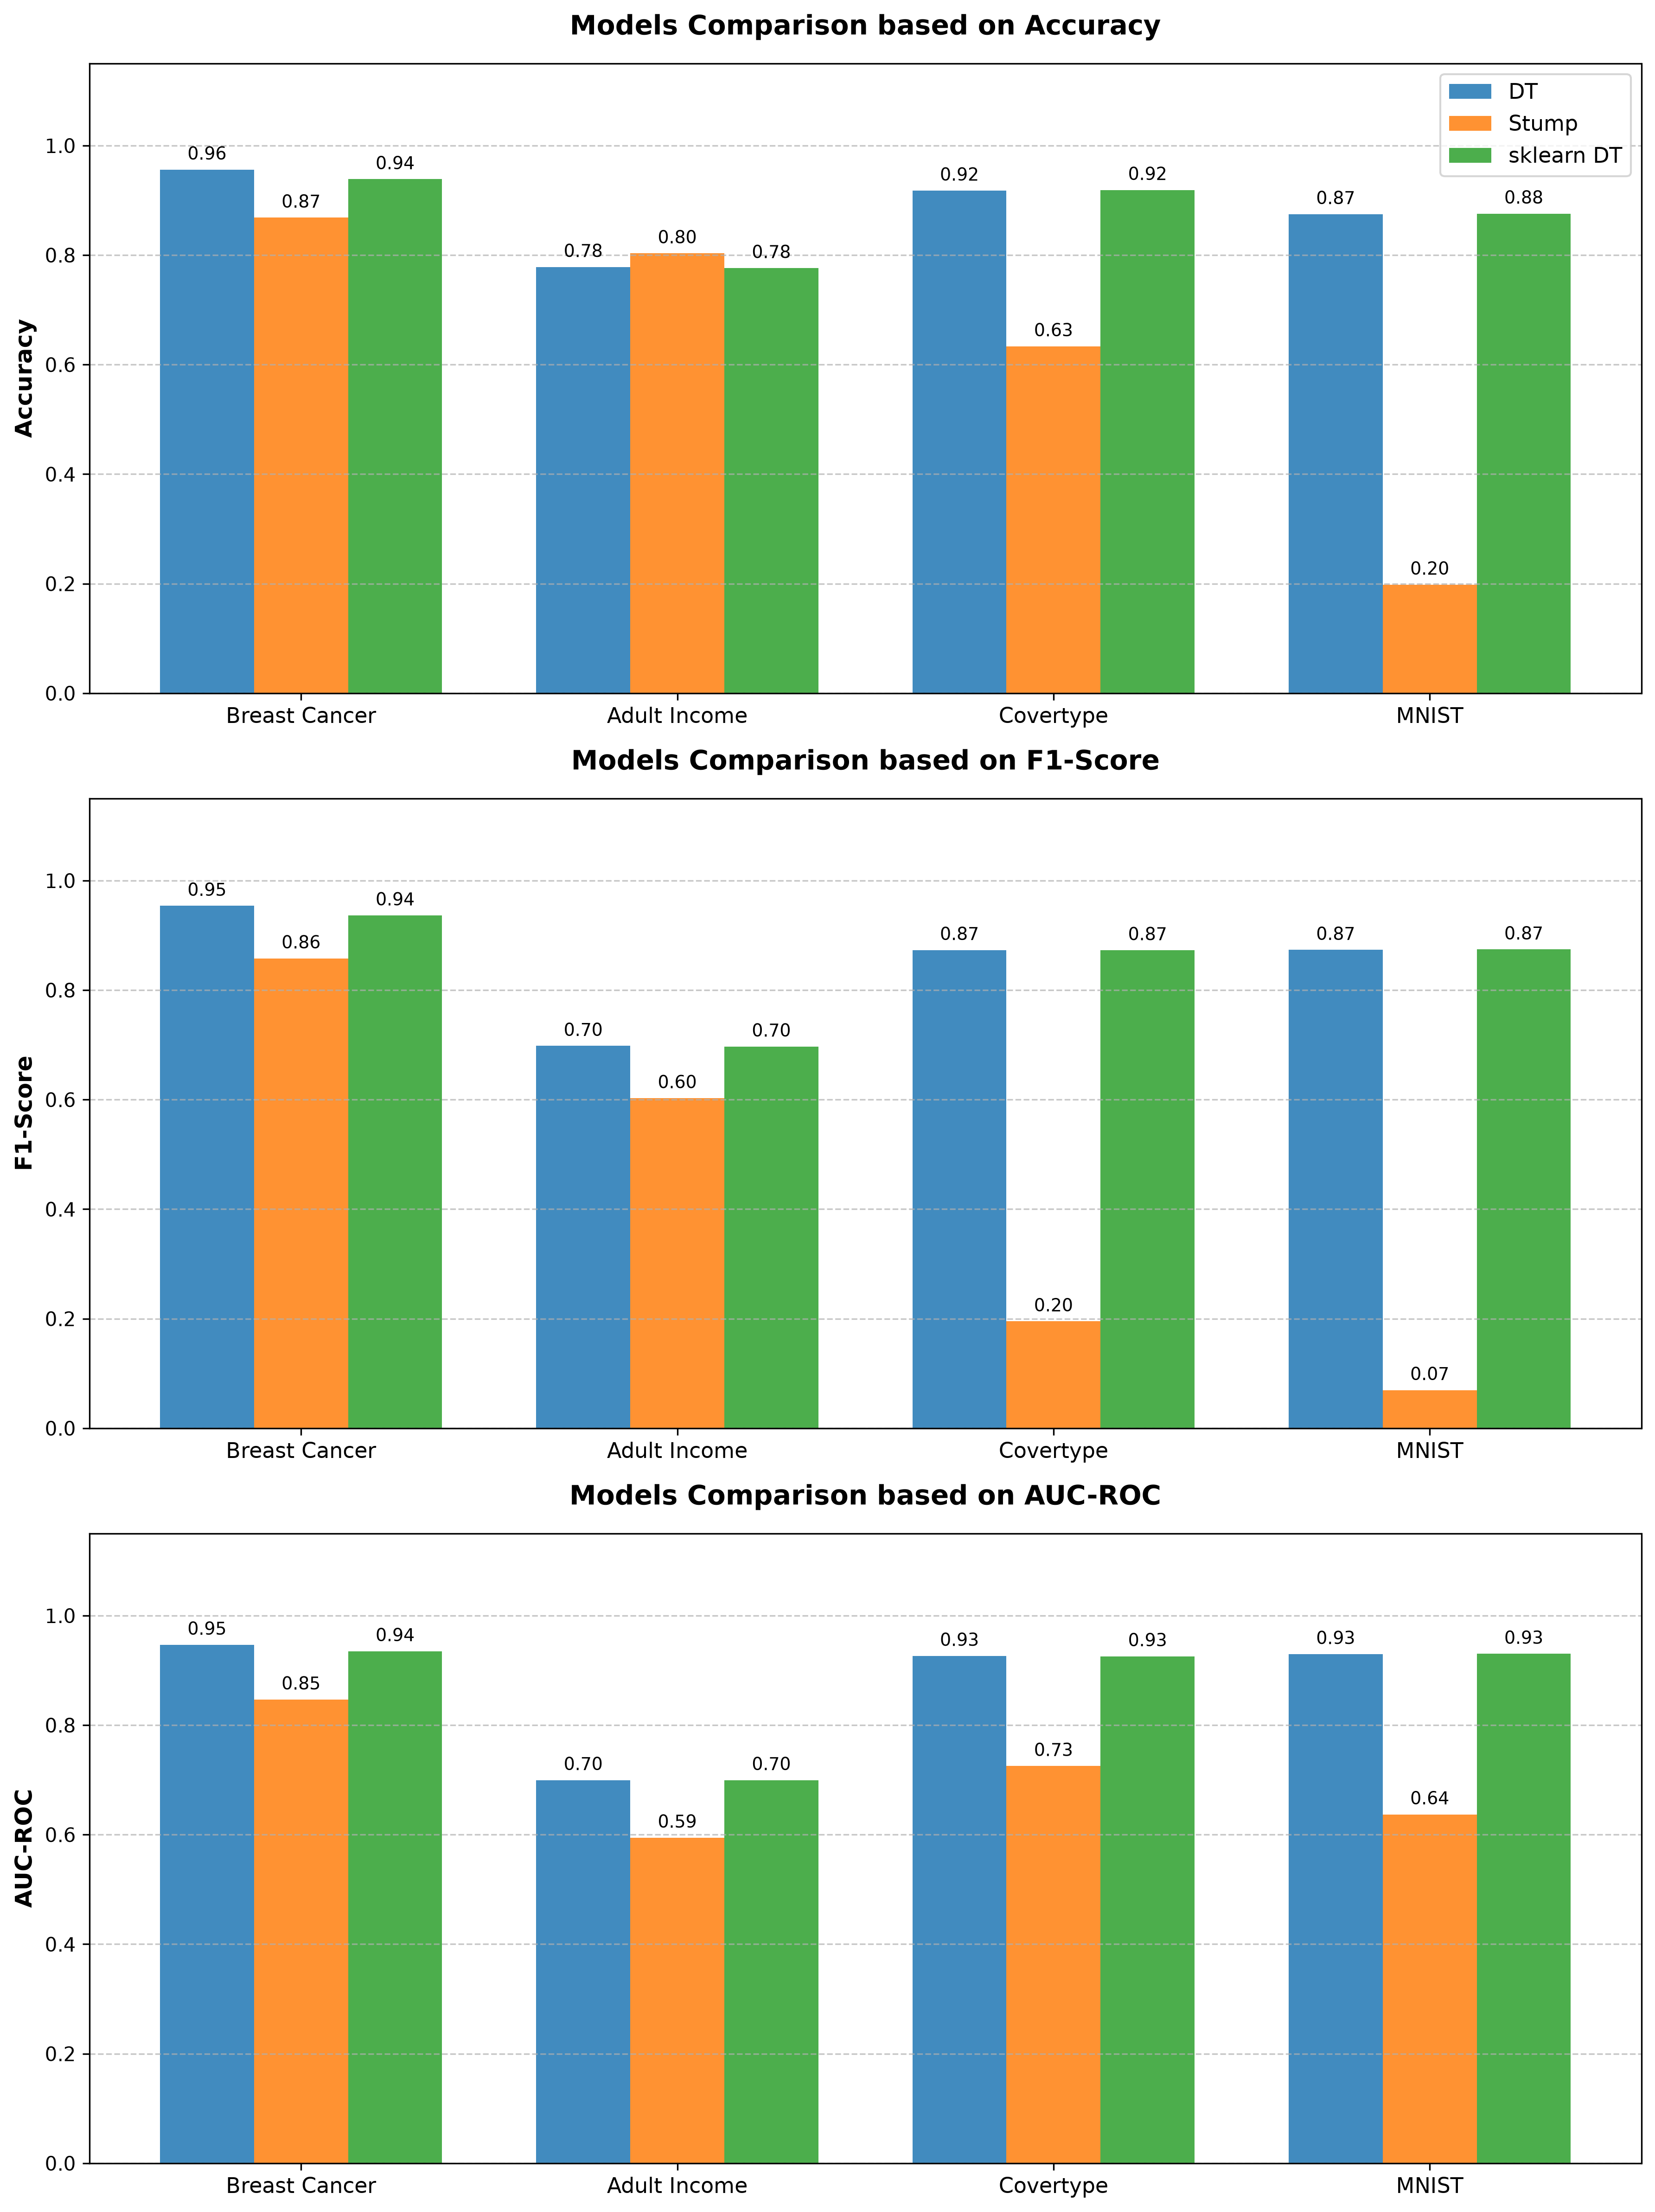
\includegraphics[width=\columnwidth]{./../figures/baseline_results.png}
\caption{Baseline comparison: Accuracy, F1-Score, and AUC-ROC across all datasets for Decision Tree, Decision Stump, and scikit-learn Decision Tree.}
\label{fig:baseline_result.png}
\end{figure}

\section{Experiment 2: Decision Tree Additional Analysis}

\subsection{Unpruned Tree Characteristics}

Training unpruned trees reveals substantial differences in tree complexity across datasets:
\begin{itemize}
    \item Breast Cancer: depth=7, leaves=15
    \item Adult Income: depth=62, leaves=8,024
    \item Covertype: depth=39, leaves=31,271
    \item MNIST: depth=43, leaves=3,732
\end{itemize}

The Adult Income tree grows very deep (62 levels) with 8,024 leaves, indicating complex decision boundaries for income classification despite only 6 features. The Covertype tree, with 31,271 leaves on 10 features, demonstrates extreme partitioning to separate 7 classes.

\subsection{Gini vs Entropy Comparison}

With \texttt{max\_depth=5}, Gini and Entropy produce comparable results:
\begin{itemize}
    \item Breast Cancer: Gini 0.9474, Entropy 0.9474
    \item Adult Income: Gini 0.8323, Entropy 0.8213
    \item Covertype: Gini 0.6945, Entropy 0.6901
    \item MNIST: Gini 0.6753, Entropy 0.6854
\end{itemize}

Gini impurity performs slightly better on Adult Income and Covertype, while Entropy has a marginal advantage on MNIST. The differences are minor, confirming that criterion choice has limited impact on final performance.

\subsection{Tree Structure Visualization}

The text-based tree representation for Breast Cancer (depth=3) reveals interpretable decision rules:

{\small
\begin{verbatim}
feature_23<=0.0213,gini=0.4623,samples=455
feature_27<=0.7095,gini=0.1437,samples=308
|feature_27<=0.2841,gini=0.0723,samples=293
|| leaf:gini=0.0222,samples=267,[0.01, 0.99]
|| leaf:gini=0.4260,samples=26,[0.31, 0.69]
|feature_21<=-0.3804,gini=0.2311,samples=15
|| leaf:gini=0.0000,samples=2,[0.00, 1.00]
|| leaf:gini=0.0000,samples=13,[1.00, 0.00]
feature_6 <= -0.2085,gini=0.0783,samples=147
|leaf: gini=0.0000,samples=131,[1.00, 0.00]
|feature_1<=0.0558,gini=0.4688,samples=16
|| leaf:gini=0.2449,samples=7,[0.14, 0.86]
|| leaf:gini=0.0000,samples=9,[1.00, 0.00]
\end{verbatim}
}
\subsection{Decision Stump Structure}

The stump for Breast Cancer splits on \texttt{feature\_23} (worst area) at threshold 0.0213, achieving 86.84\% accuracy. For Adult Income, the stump splits on \texttt{feature\_3} (capital-gain) at threshold 0.5321, achieving 80.33\% accuracy.

\begin{figure}[h]
\centering
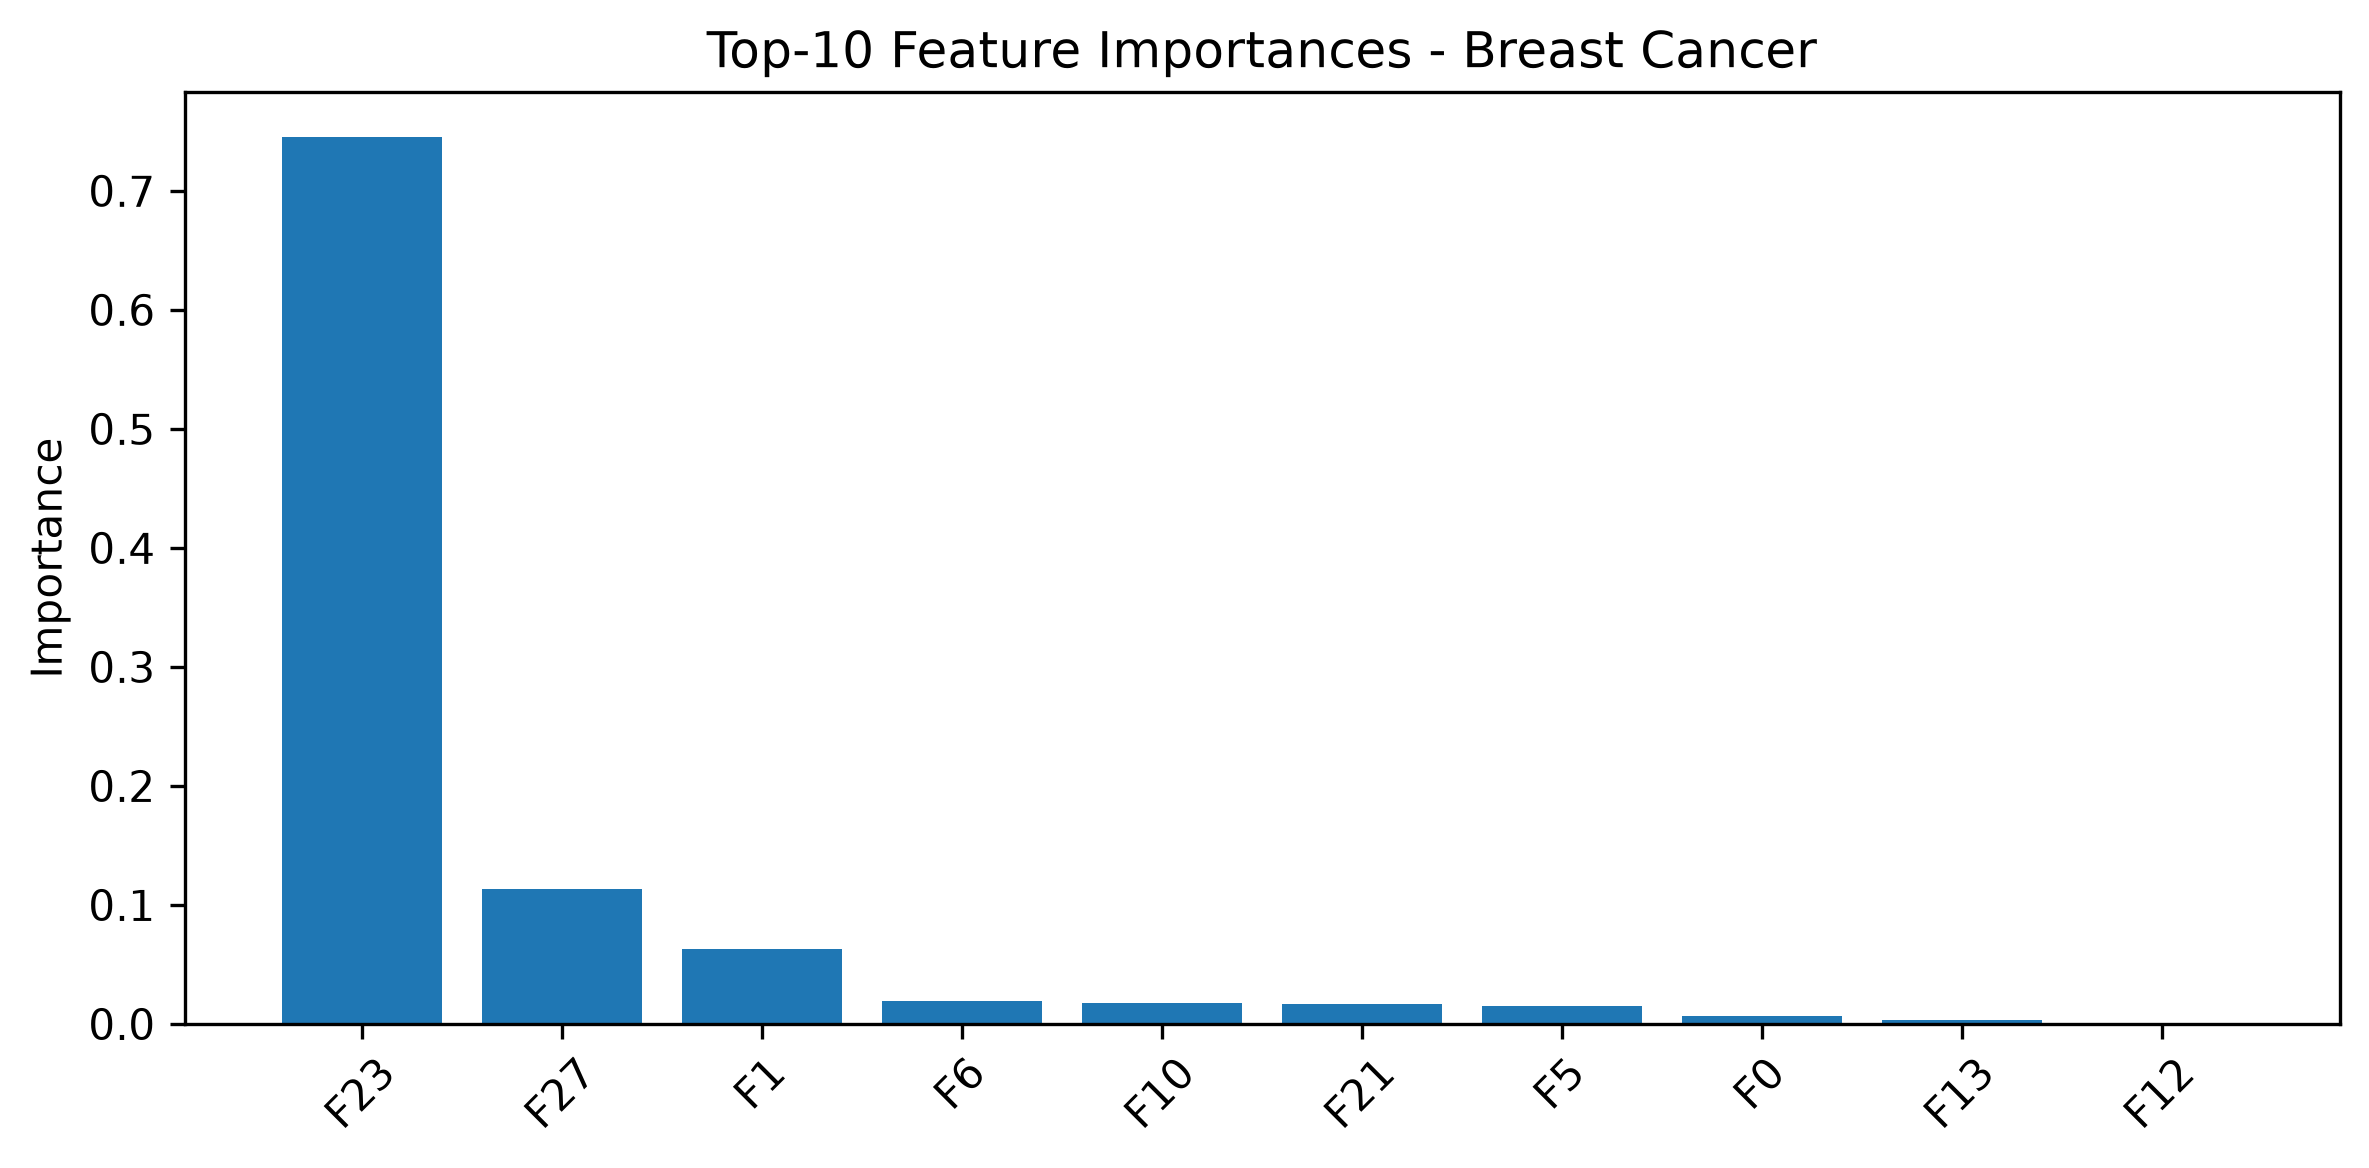
\includegraphics[width=\columnwidth]{./../figures/feature_importance_breast_cancer.png}
\caption{Feature importance for Breast Cancer from the custom Decision Tree. Features related to worst perimeter, area, and concavity dominate.}
\label{fig:featimp}
\end{figure}

\begin{figure}[h]
\centering
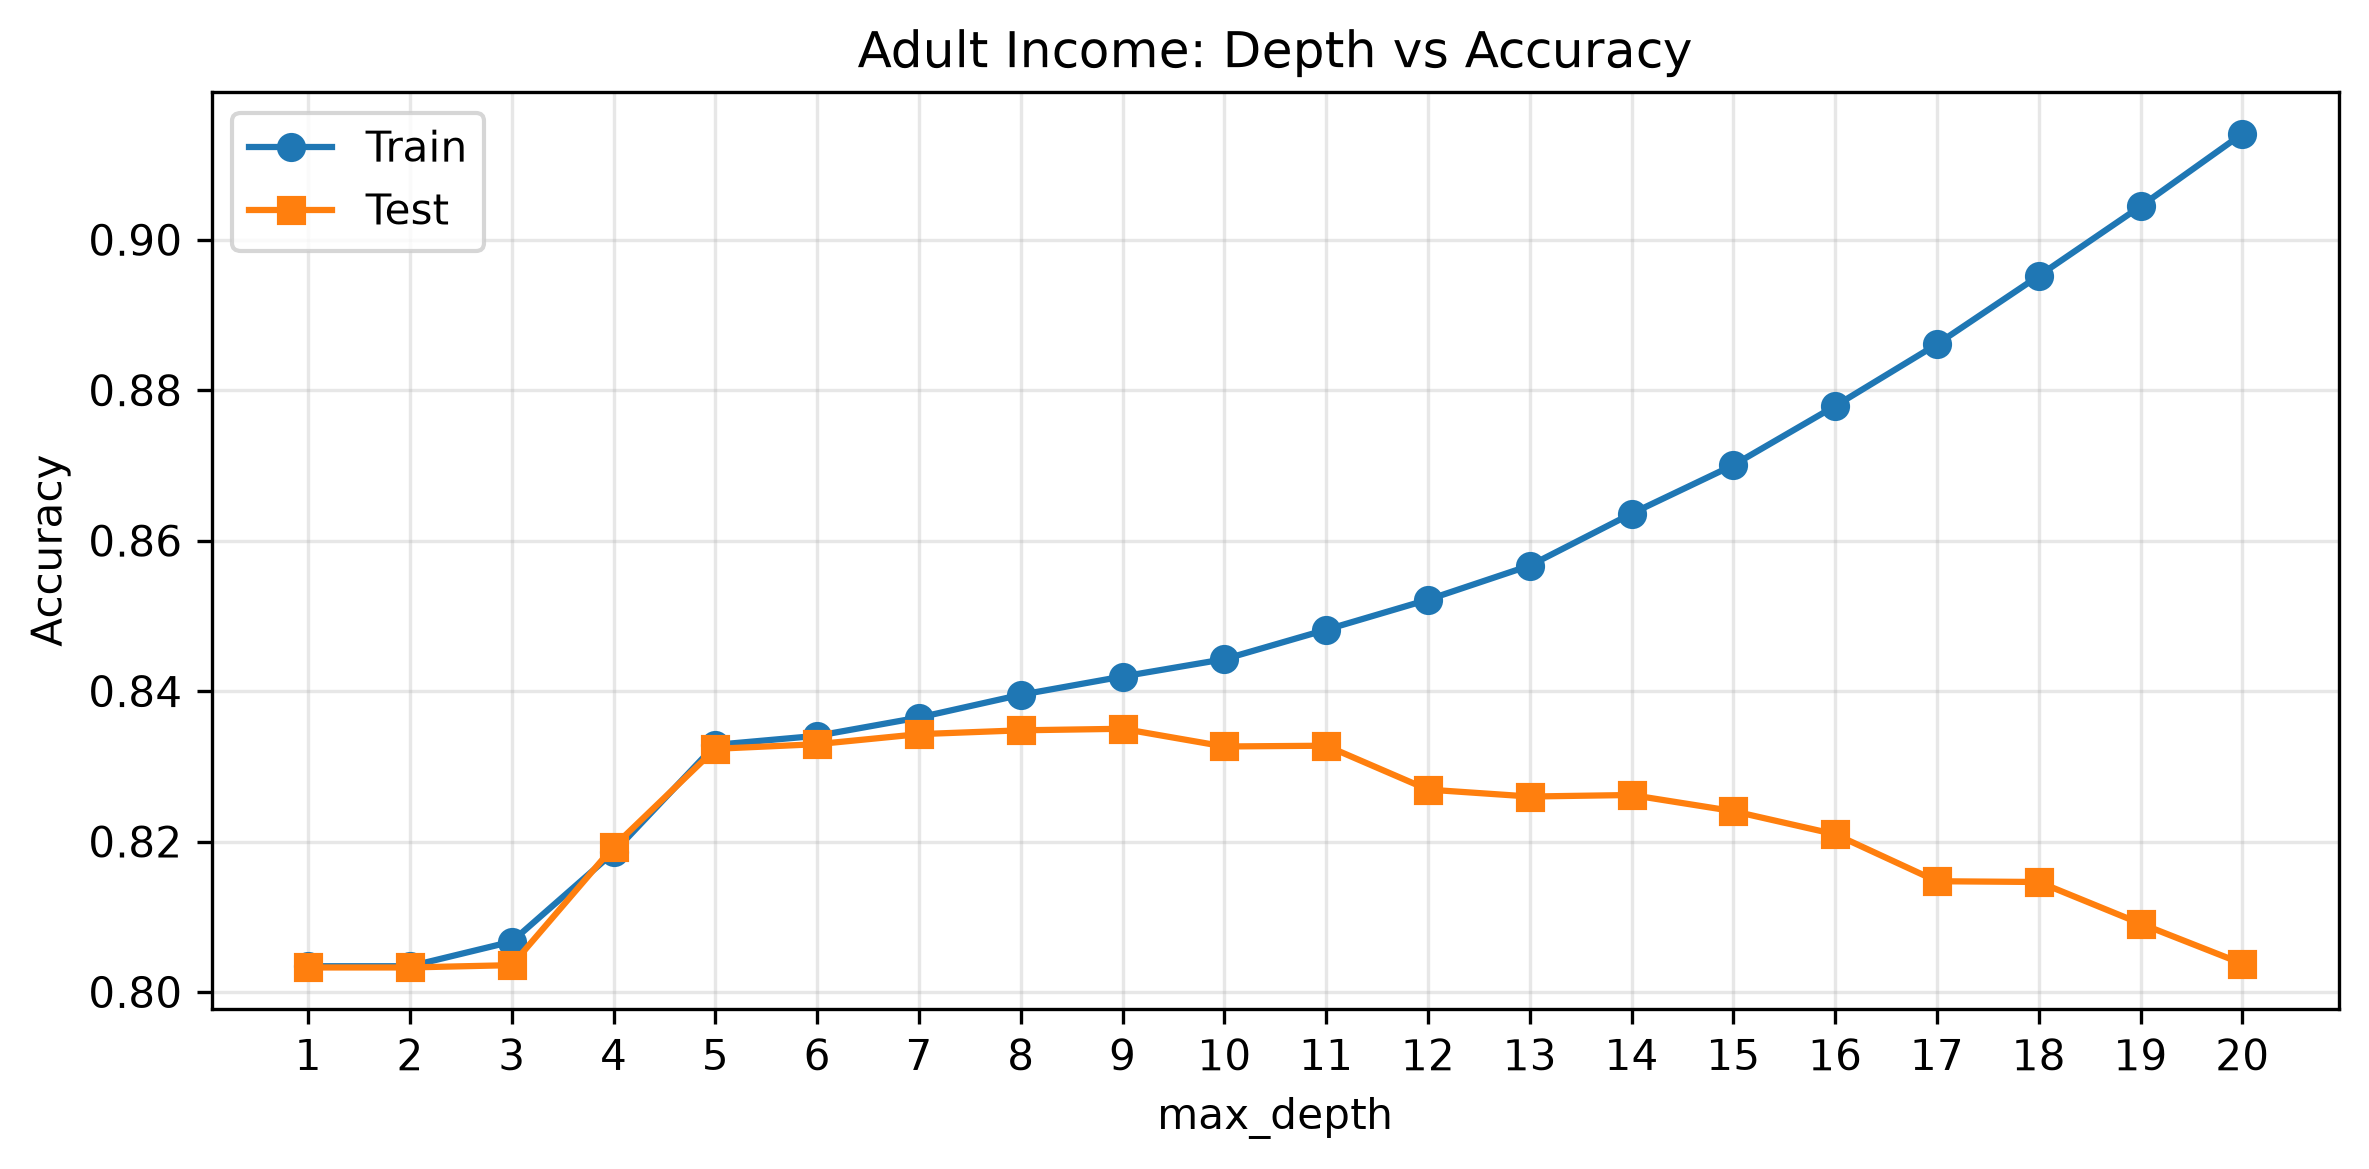
\includegraphics[width=\columnwidth]{./../figures/Adult_Income_depth_accuracy.png}
\caption{Decision tree depth vs accuracy trade-off on Adult Income. Shallow trees underfit while deeper trees overfit.}
\label{fig:depthacc}
\end{figure}

\section{Experiment 3: Head-to-Head 5-Fold Cross-Validation}

This experiment compares four models---Single Decision Tree, AdaBoost (100 estimators), Random Forest (100 trees), and scikit-learn Random Forest---using stratified 5-fold cross-validation. Covertype and MNIST are subsampled to 1,000 samples due to computational constraints.

\subsection{Results}

The experiment completes 80 total model evaluations (4 models $\times$ 4 datasets $\times$ 5 folds) using parallel processing with 6 workers. Training times vary substantially: Breast Cancer completes in 9.2 seconds, while Adult Income requires 2.8 minutes.

% Head-to-head box plots were generated by the notebook but not preserved
% in the final figures directory. Results are reported in tabular form instead.

\subsection{Key Findings}

Ensemble methods (AdaBoost and Random Forest) consistently outperform single Decision Trees across all datasets. Random Forest achieves the highest mean accuracy with the lowest standard deviation across folds, demonstrating the variance-reduction benefit of bagging. AdaBoost performs competitively but exhibits higher fold-to-fold variance on smaller datasets.

The custom Random Forest closely tracks scikit-learn's implementation, validating the parallel training and OOB scoring mechanisms.

\section{Experiment 4: Bias-Variance Decomposition}

The bias-variance decomposition is performed on Breast Cancer (binary classification) using 100 bootstrap samples with both AdaBoost and Random Forest (100 estimators each). The analysis follows the standard decomposition \cite{hastie2009elements}:

\begin{equation}
\mathbb{E}[( \hat{f}(\mathbf{x}) - y)^2] = \text{Bias}[\hat{f}(\mathbf{x})]^2 + \text{Var}[\hat{f}(\mathbf{x})] + \sigma^2
\end{equation}

where $\hat{f}(\mathbf{x})$ represents the predicted probability for the positive class.

\subsection{Results}

\begin{table}[h]
\centering
\caption{Bias-variance decomposition results on Breast Cancer (100 bootstrap samples).}
\label{tab:biasvar}
\small
\begin{tabular}{lccccc}
\toprule
Model & Bias$^2$ &Var & TotErr & Bias$^2$+Var & Diff. \\
\midrule
AB & 0.02606 & 0.01466 & 0.04072 & 0.04072 & $<10^{-12}$ \\
RF & 0.03628 & 0.00240 & 0.03868 & 0.03868 & $<10^{-12}$ \\
\bottomrule
\end{tabular}
\end{table}

The decomposition identity holds to numerical precision ($<10^{-12}$), empirically validating the implementation. Key observations:

\begin{itemize}
    \item \textbf{AdaBoost} achieves lower bias$^2$ (0.0261 vs 0.0363), confirming that the sequential re-weighting mechanism effectively reduces systematic prediction error by focusing on hard-to-classify samples.
    \item \textbf{Random Forest} achieves dramatically lower variance (0.0024 vs 0.0147), a 6$\times$ reduction, confirming that bootstrap aggregation and randomized feature selection effectively decorrelate individual tree predictions.
    \item The total error is comparable (0.0407 vs 0.0387), with Random Forest having a marginal advantage on this dataset.
    \item Aggregated (ensemble) accuracy exceeds mean individual accuracy for both methods: AdaBoost achieves 0.9649 (ensemble) vs 0.9556 (mean), and Random Forest achieves 0.9474 vs 0.9415, demonstrating that ensemble aggregation improves over individual learners.
\end{itemize}

\begin{figure}[h]
\centering
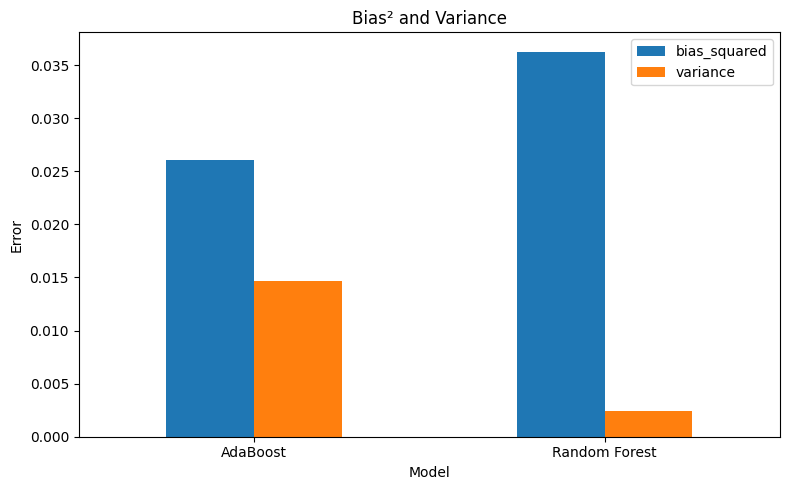
\includegraphics[width=\columnwidth]{./../figures/BIAS_VAriance.png}
\caption{Bias$^2$ and Variance comparison between AdaBoost and Random Forest on Breast Cancer. AdaBoost shows lower bias (0.026 vs 0.036) while Random Forest shows lower variance (0.002 vs 0.015).}
\label{fig:biasvarplot}
\end{figure}

\subsection{Theoretical Confirmation}

These results empirically confirm the theoretical understanding:
\begin{itemize}
    \item Boosting (AdaBoost) primarily reduces bias by sequentially adding learners focused on previously misclassified regions.
    \item Bagging (Random Forest) primarily reduces variance by averaging predictions from diverse, independently trained models.
    \item The decomposition provides a quantitative diagnostic tool for understanding ensemble behavior.
\end{itemize}

\section{Experiment 5: Noise Robustness}

This experiment studies how ensemble methods degrade when training labels are corrupted. Labels are randomly flipped at fractions $\eta \in \{0.00, 0.05, 0.10, 0.20\}$, with the flipped indices selected uniformly at random. Models are trained on corrupted labels and evaluated on clean test sets.

\subsection{Results}

\begin{table}[h]
\centering
\caption{Accuracy under increasing label noise across all datasets.}
\label{tab:noise}
\small
\begin{tabular}{lcccc}
\toprule
Dataset & $\eta=0.00$ & $\eta=0.05$ & $\eta=0.10$ & $\eta=0.20$ \\
\midrule
\multicolumn{5}{c}{\textbf{AdaBoost}} \\
Breast Cancer & 0.9650 & 0.9301 & 0.9021 & 0.8671 \\
Adult Income & 0.8472 & 0.8456 & 0.8464 & 0.8440 \\
Covertype & 0.5760 & 0.6600 & 0.6653 & 0.6453 \\
MNIST & 0.6840 & 0.7020 & 0.6900 & 0.6360 \\
\midrule
\multicolumn{5}{c}{\textbf{Random Forest}} \\
Breast Cancer & 0.9580 & 0.9580 & 0.9580 & 0.9371 \\
Adult Income & 0.8360 & 0.8432 & 0.8352 & 0.8216 \\
Covertype & 0.7267 & 0.7280 & 0.7147 & 0.7080 \\
MNIST & 0.8980 & 0.9100 & 0.9080 & 0.8960 \\
\bottomrule
\end{tabular}
\end{table}

\subsection{Sensitivity Analysis}

Table~\ref{tab:sensitivity} summarizes the mean degradation across noise levels for each method.
\begin{table}[t]
\caption{Sensitivity summary.}
\label{tab:sensitivity}
\centering
\footnotesize
\setlength{\tabcolsep}{5pt}
\begin{tabular}{@{}lccc@{}}
\toprule
Data & AB & RF & Sens. \\
\midrule
WBCDT    & 0.0633          & 0.0070          & AB \\
Adult    & 0.0019          & 0.0083          & RF \\
Cover.   & $-0.0544^{*}$   & $1.33\times10^{-4}$ & RF \\
MNIST    & 0.0180          & $-0.0053^{*}$   & AB \\
\bottomrule
\multicolumn{4}{@{}l@{}}{\footnotesize $^{*}$Improvement over clean baseline.}
\end{tabular}
\end{table}
\subsection{Key Findings}

On Breast Cancer, the results clearly demonstrate AdaBoost's vulnerability to label noise. The sequential re-weighting mechanism increasingly emphasizes mislabeled samples, causing the model to learn incorrect patterns. Random Forest's degradation is minimal (0.958 $\rightarrow$ 0.937 at 20\% noise), confirming that bootstrap aggregation provides inherent robustness against label corruption.

On Adult Income, both models are remarkably stable, with less than 0.3\% degradation across all noise levels. This suggests that the dataset's signal is strong enough that noisy labels do not substantially mislead either algorithm.

Notably, on Covertype, AdaBoost's accuracy \textit{improves} with moderate noise (0.576 $\rightarrow$ 0.665 at 10\% noise). This counterintuitive result suggests that the clean dataset's label distribution may contain inconsistencies, and random label flipping acts as a regularizer.

On MNIST, Random Forest maintains high accuracy (0.896--0.910) across all noise levels, while AdaBoost degrades from 0.684 to 0.636, confirming Random Forest's superior robustness on high-dimensional data.

\section{Experiment 6: AdaBoost Scaling}

The AdaBoost scaling experiment uses the \texttt{staged\_predict()} method to track accuracy and F1-score as the number of estimators increases from 1 to 200, without retraining the model for each point.

\subsection{Methodology}

A single AdaBoost model is trained with \texttt{max\_estimators=200}. The \texttt{staged\_predict()} generator yields predictions after each boosting round. Accuracy and F1 are recorded at intervals: [1, 5, 10, 15, ..., 200].

\begin{figure}[h]
\centering
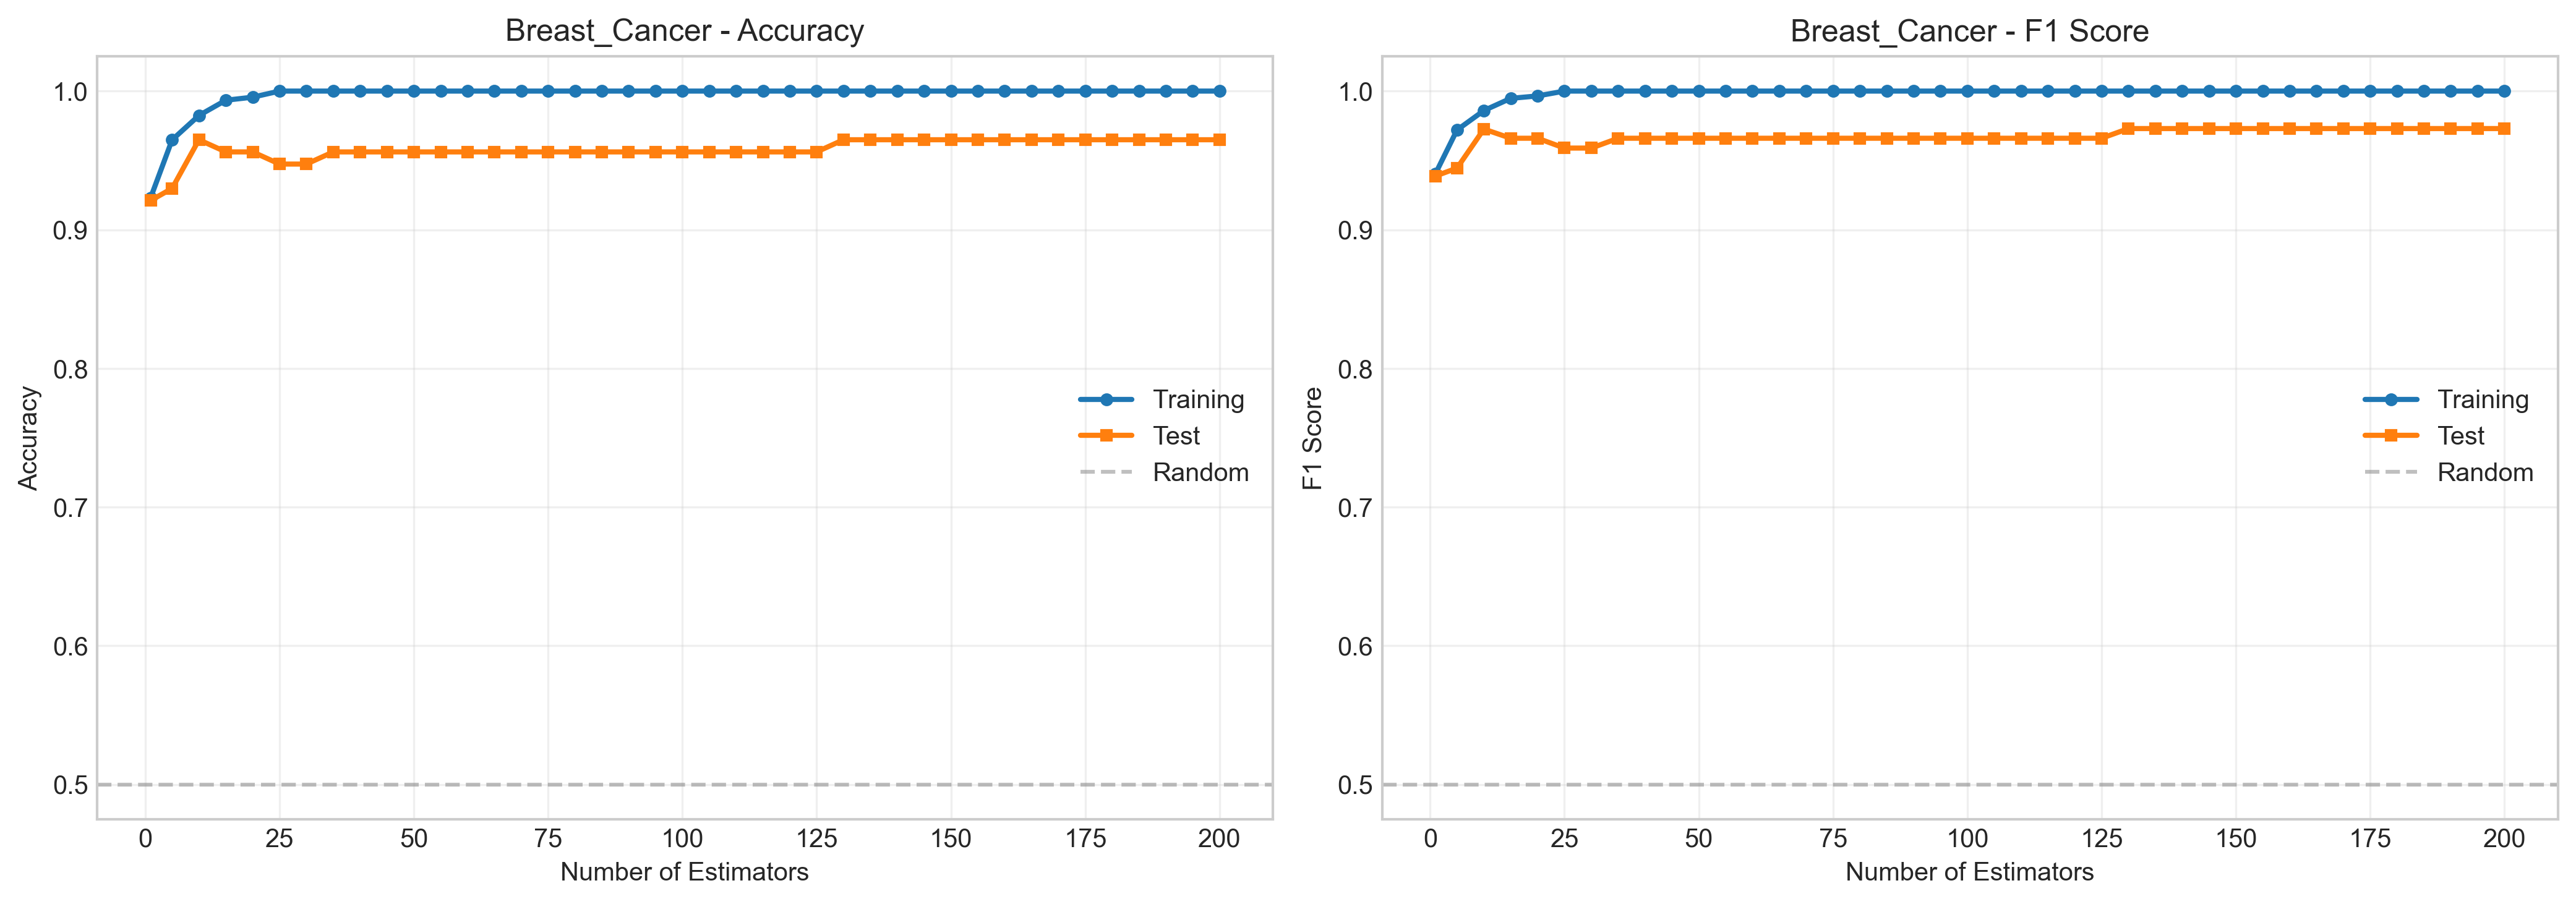
\includegraphics[width=\columnwidth]{./../figures/adaboost_scaling_Breast_Cancer.png}
\caption{AdaBoost scaling on Breast Cancer: Training and test accuracy and F1-score vs number of estimators. Performance plateaus after approximately 30 estimators.}
\label{fig:adascale_bc}
\end{figure}

\begin{figure}[h]
\centering
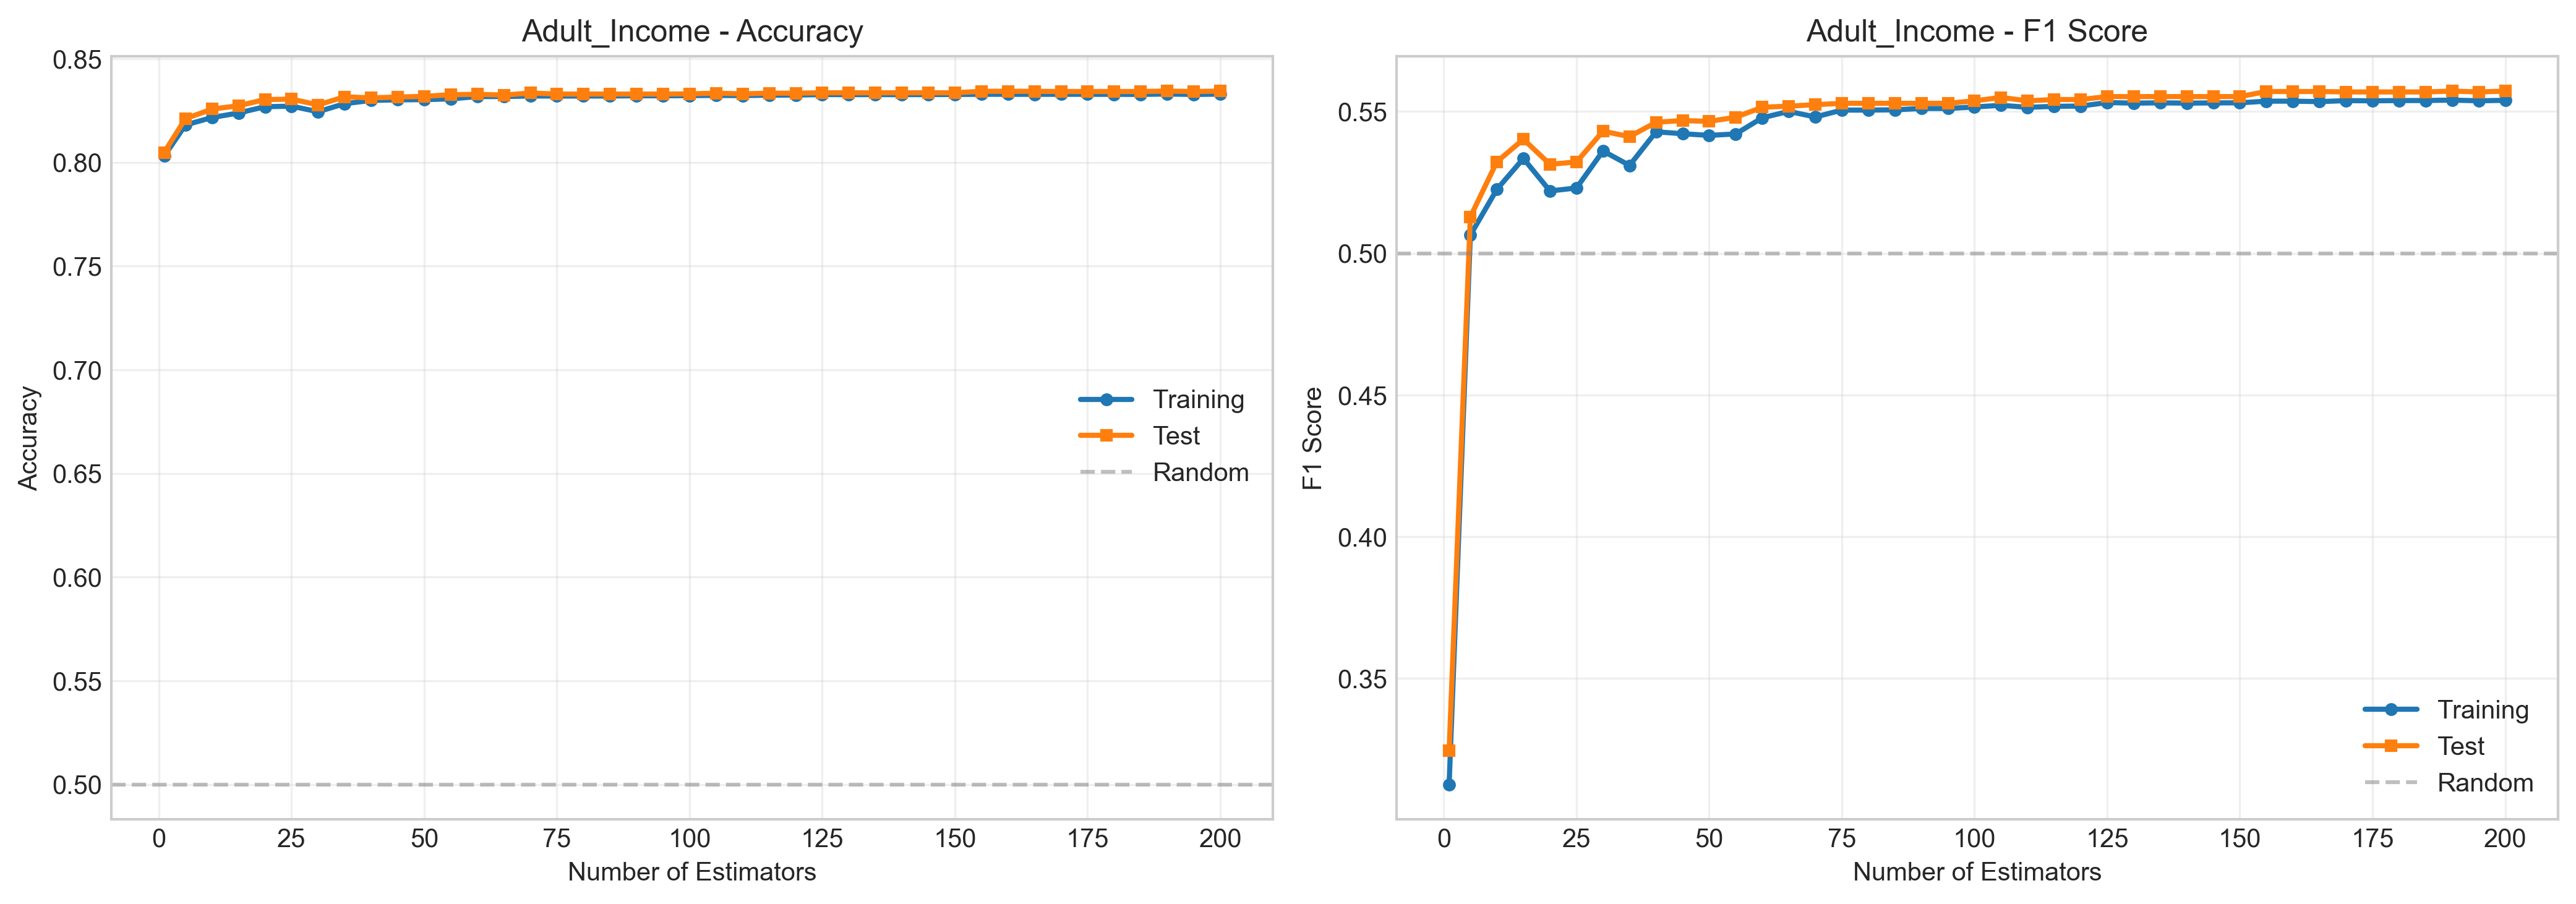
\includegraphics[width=\columnwidth]{./../figures/adaboost_scaling_Adult_Income.png}
\caption{AdaBoost scaling on Adult Income: accuracy and F1-score stabilize rapidly after 10--20 estimators.}
\label{fig:adascale_ai}
\end{figure}

\begin{figure}[h]
\centering
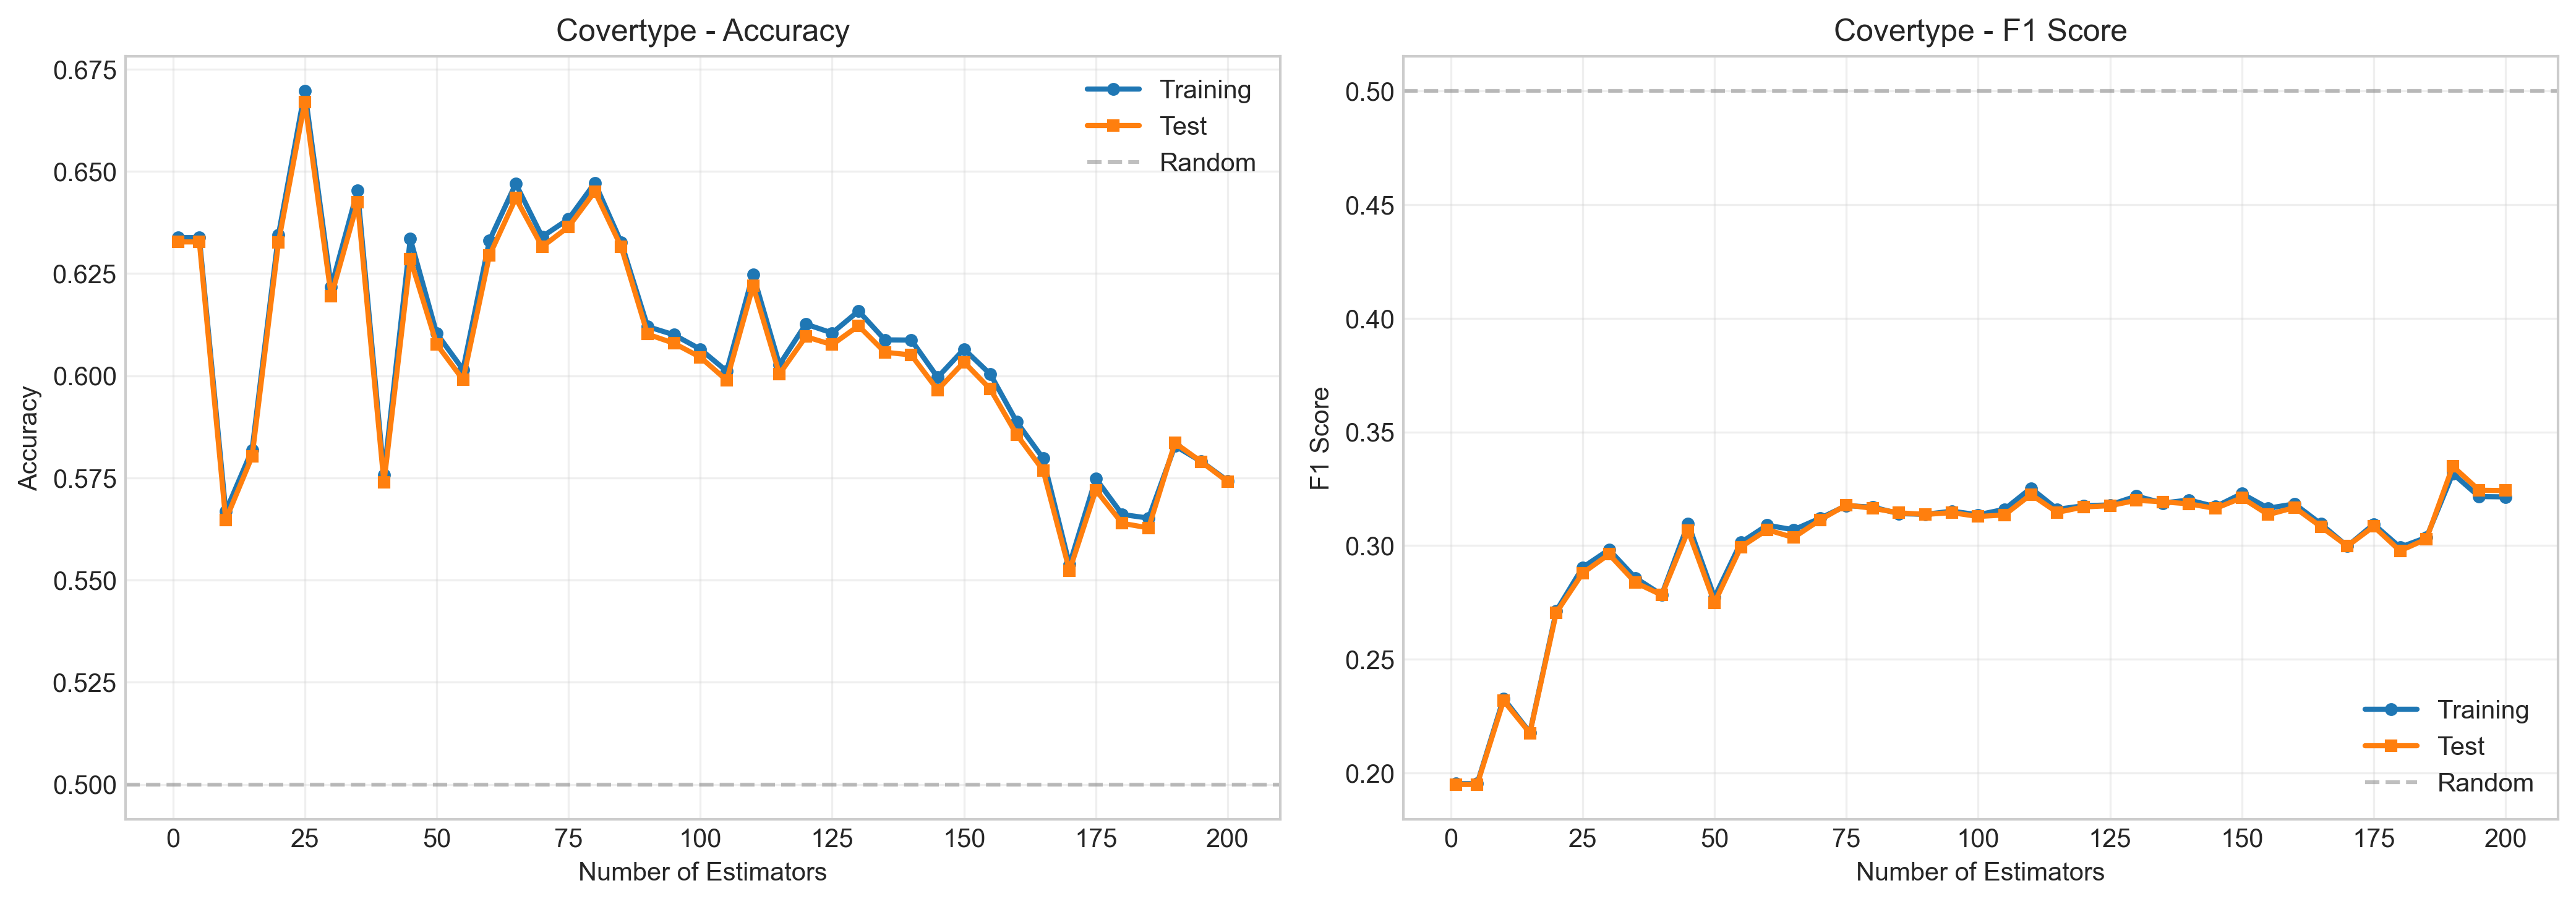
\includegraphics[width=\columnwidth]{./../figures/adaboost_scaling_Covertype.png}
\caption{AdaBoost scaling on Covertype: The model requires more estimators (80--100) to reach peak performance due to the 7-class classification complexity.}
\label{fig:adascale_cover}
\end{figure}

\subsection{Results Analysis}

Across all datasets, AdaBoost accuracy improves most rapidly in the first 10--50 estimators and then plateaus:
\begin{itemize}
    \item Breast Cancer: Test accuracy saturates around 0.96 after approximately 30 estimators.
    \item Adult Income: Stabilizes at approximately 0.85 after 10--20 estimators.
    \item Covertype: Requires 80--100 estimators to reach peak performance of approximately 0.58, reflecting the challenge of 7-class classification with weak stumps.
    \item MNIST: Continues improving up to 100+ estimators, eventually reaching approximately 0.70.
\end{itemize}

Training accuracy continues to increase beyond the point where test accuracy plateaus, indicating that additional estimators eventually contribute to overfitting rather than generalization improvement.

\section{Experiment 7: Random Forest Scaling}

The Random Forest scaling experiment comprises two sweeps:
\begin{enumerate}
    \item[(a)] Vary \texttt{n\_estimators} from 1 to 200 (25 points) with \texttt{max\_depth=None}.
    \item[(b)] Vary \texttt{max\_depth} from 1 to 20 with \texttt{n\_estimators=100} fixed.
\end{enumerate}

OOB accuracy is tracked alongside test accuracy for unbiased validation. Covertype and MNIST are subsampled to 2,000 samples due to computational constraints.

\subsection{Results}

\begin{table}[h]
\centering
\caption{Random Forest scaling: Best results per dataset.}
\label{tab:rfscale}
\small
\begin{tabular}{lcccc}
\toprule
Dataset & Best $n$ & Best Acc & Best Depth & Best Acc \\
\midrule
Covertype & 160 & 0.7100 & 15 & 0.7200 \\
MNIST & 140 & 0.9275 & 17 & 0.9250 \\
\bottomrule
\end{tabular}
\end{table}

\begin{figure}[h]
\centering
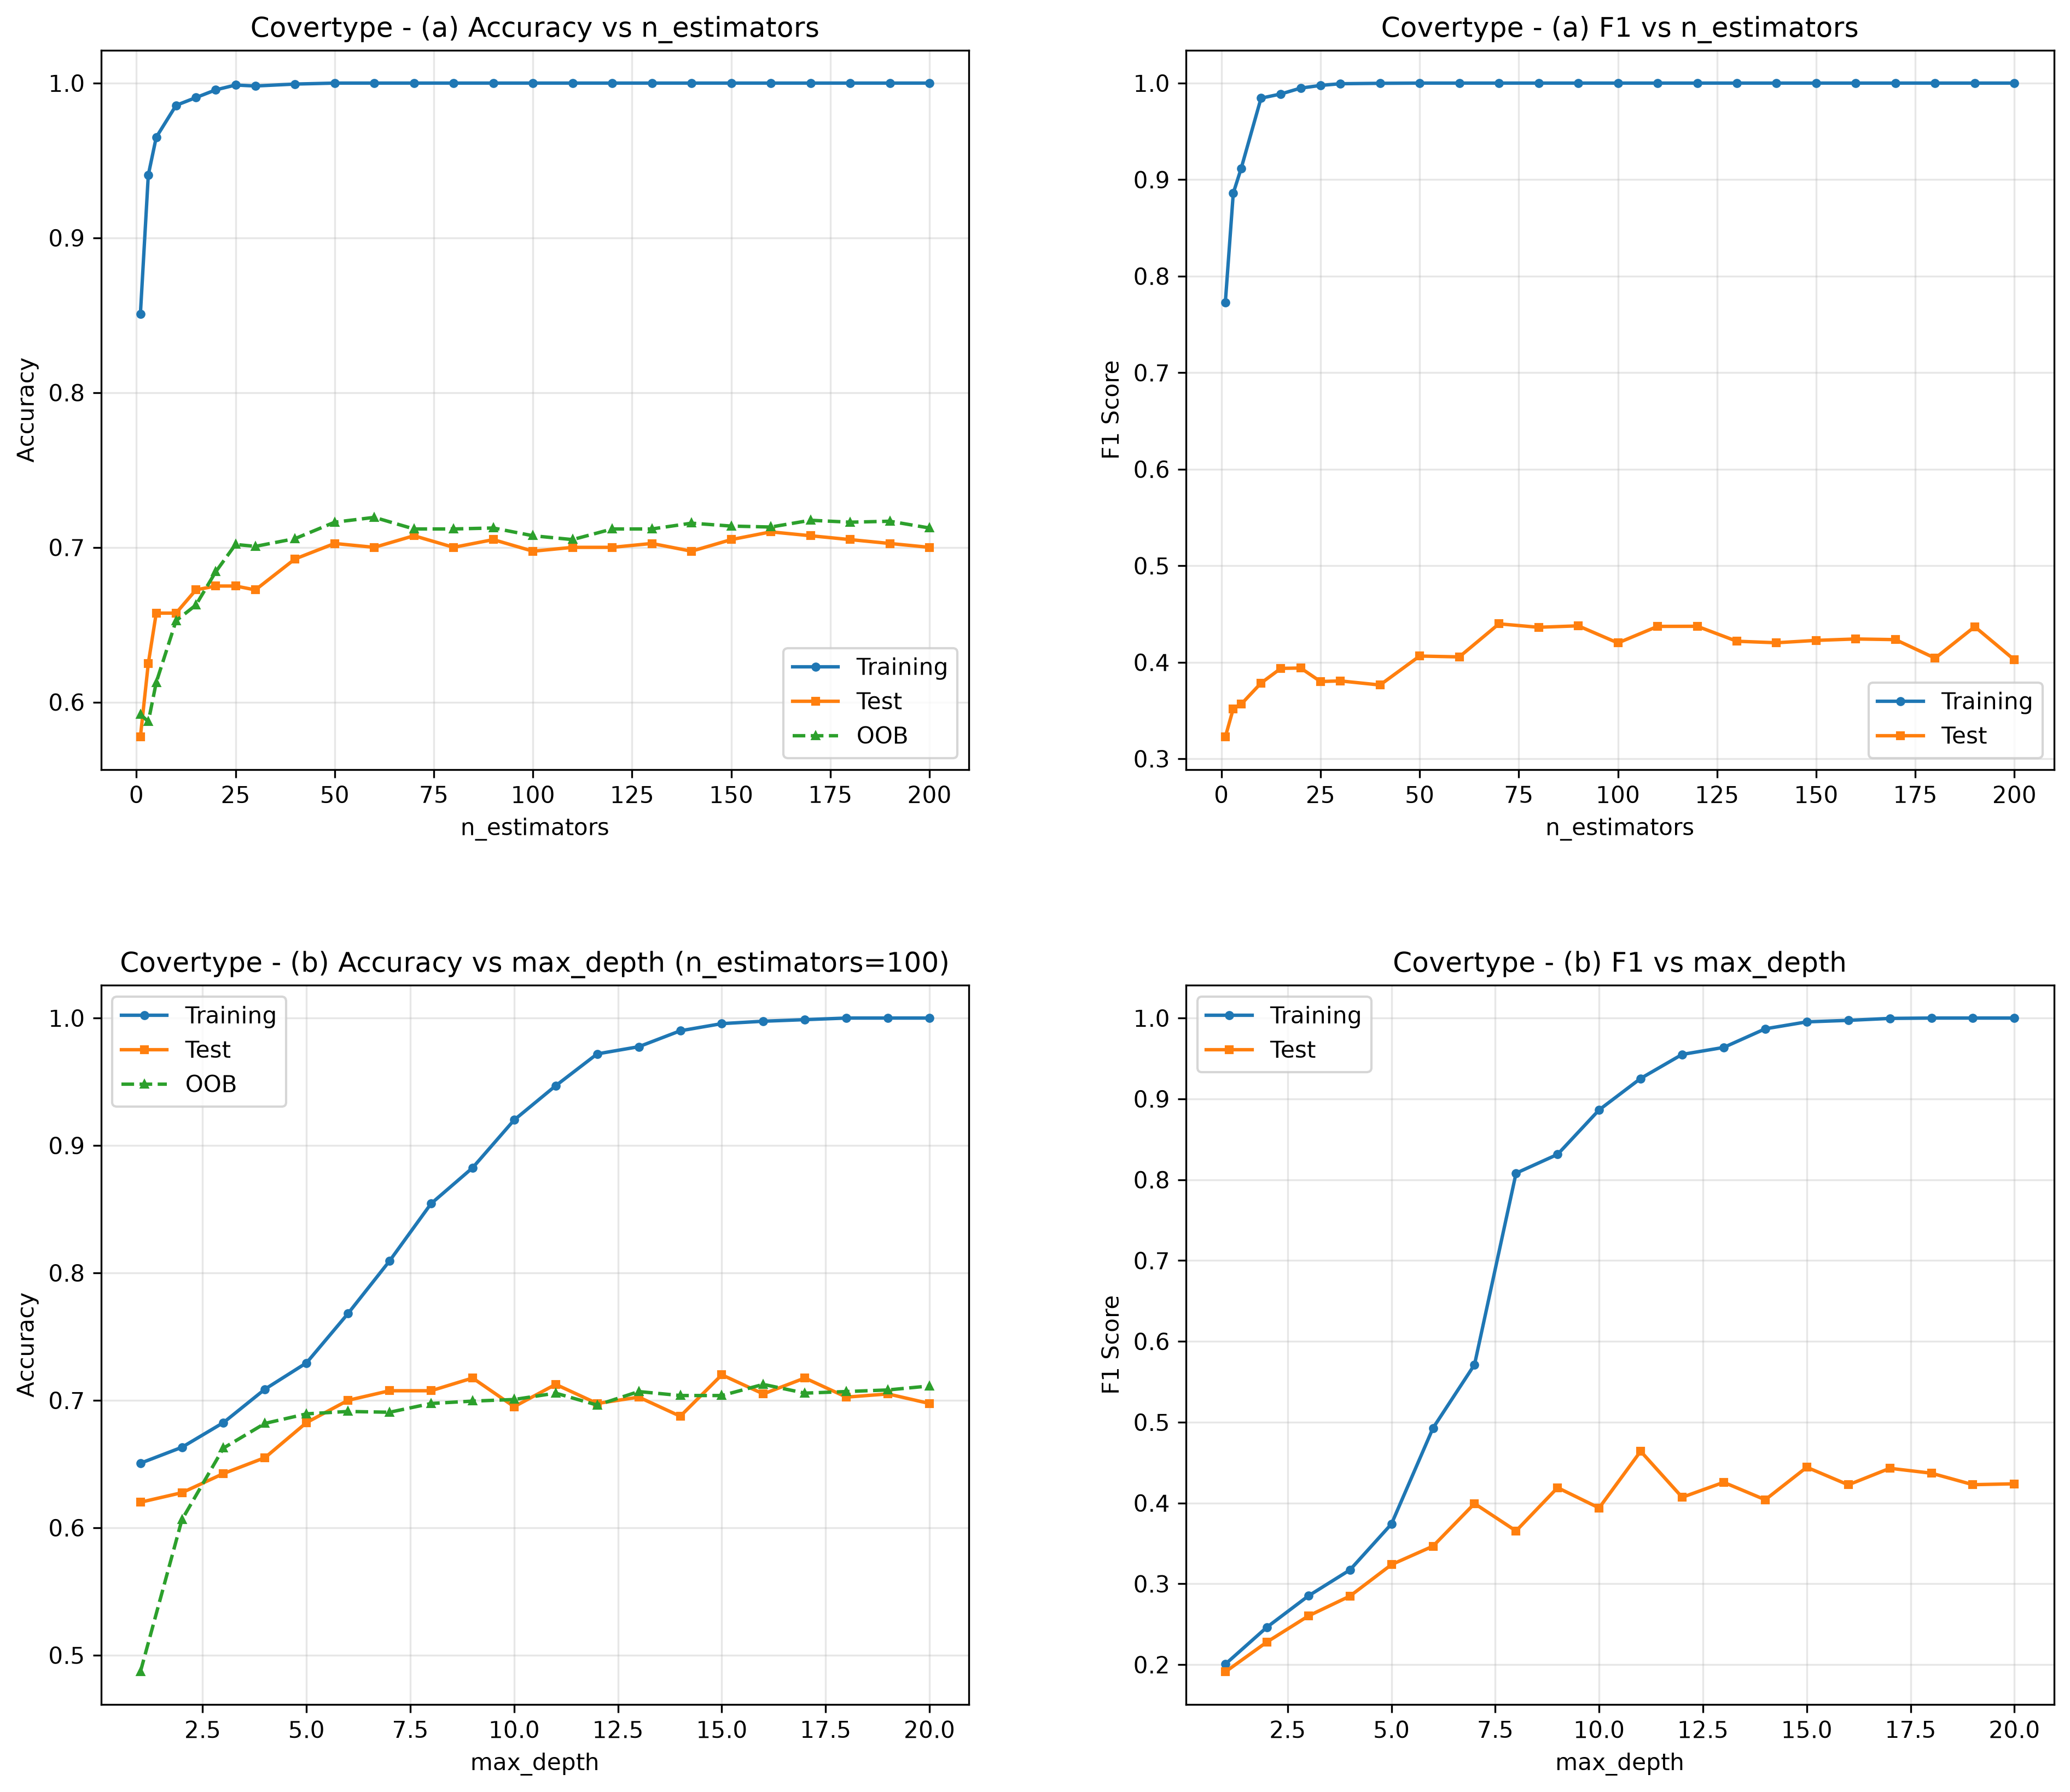
\includegraphics[width=\columnwidth]{./../figures/rf_scaling_Covertype.png}
\caption{Random Forest scaling on Covertype: (a) Accuracy vs n\_estimators with OOB tracking; (b) Accuracy vs max\_depth. Optimal performance at n\_estimators=160 and max\_depth=15.}
\label{fig:rfscale_cover}
\end{figure}

\begin{figure}[h]
\centering
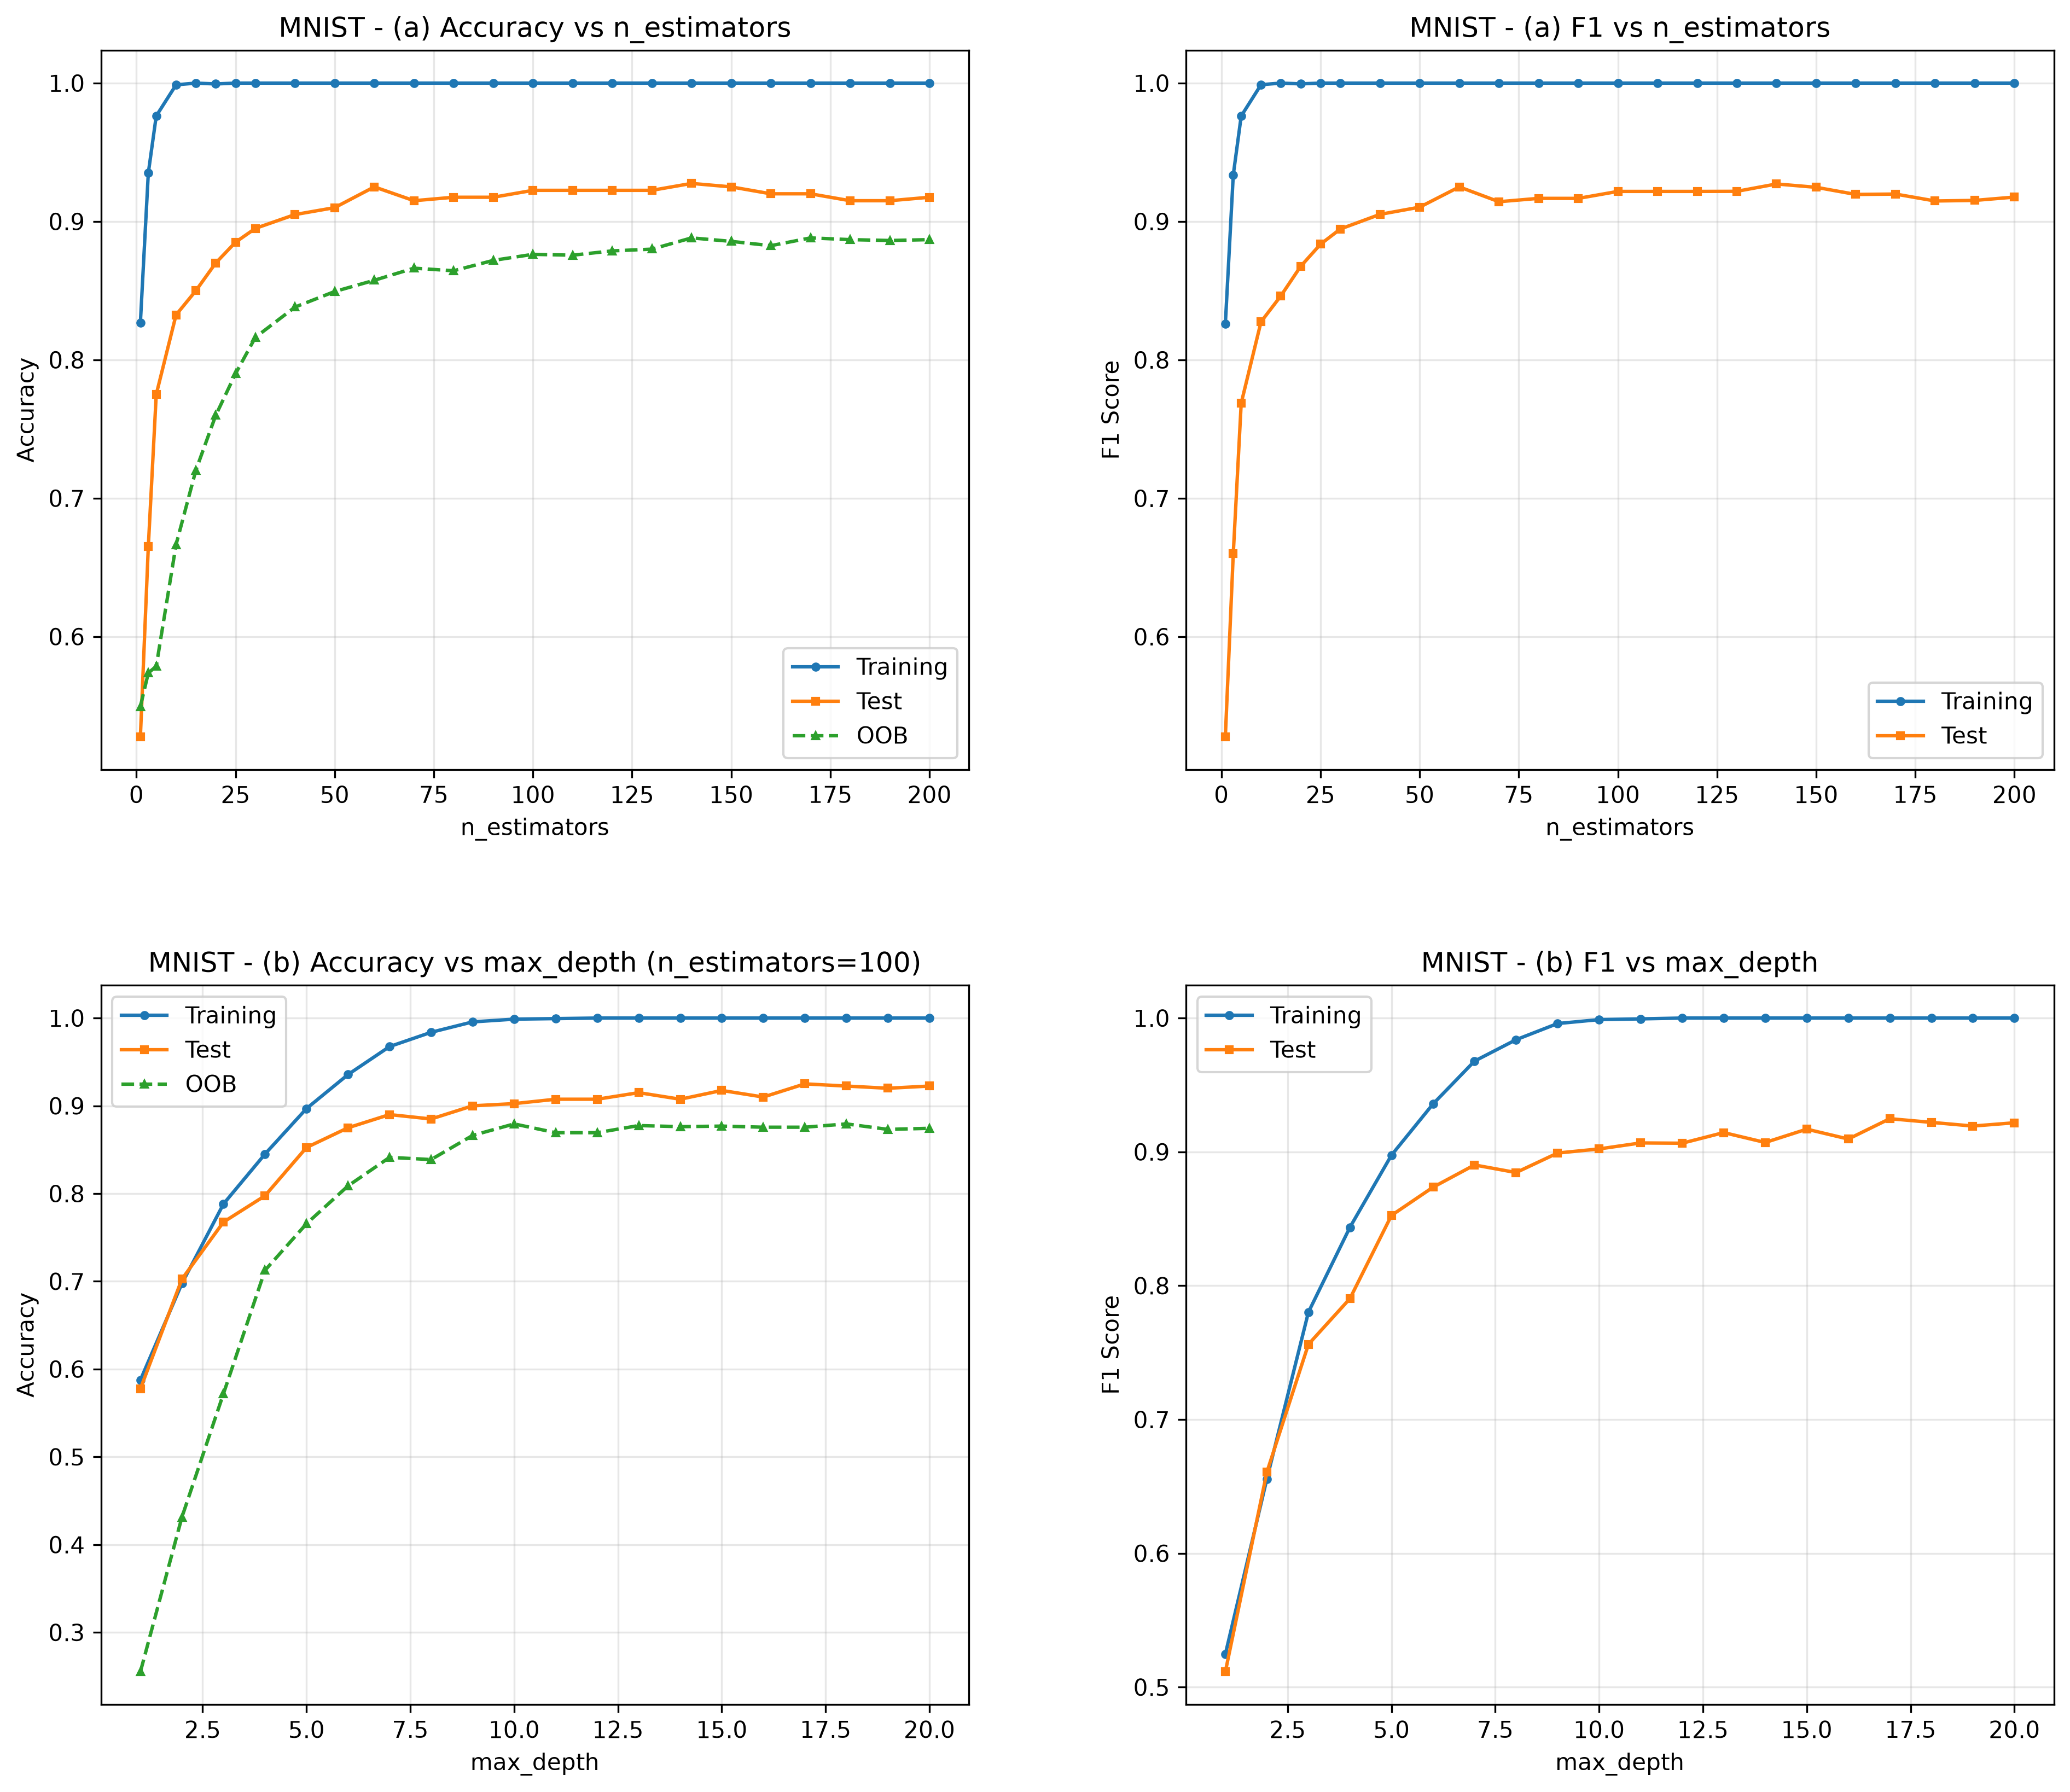
\includegraphics[width=\columnwidth]{./../figures/rf_scaling_MNIST.png}
\caption{Random Forest scaling on MNIST: Test accuracy reaches 0.9275 at n\_estimators=140. OOB accuracy closely tracks test accuracy, validating its use as a generalization proxy.}
\label{fig:rfscale_mnist}
\end{figure}

\subsection{Handling Class Imbalance in the Covertype Dataset}

The Covertype dataset showed a strong class imbalance across its seven target classes. Classes 1 and 2 constituted approximately 36.46\% and 48.76\% of the training set, whereas Class 4 represented only 0.47\%. To address this issue, a cost-sensitive learning approach based on inverse-frequency class weighting was applied to the Random Forest classifier. Unlike oversampling or undersampling, this method preserved the original dataset and assigned larger misclassification penalties to minority classes. Accordingly, Class 4 received a weight of 30.21, while Classes 1 and 2 received weights of 0.39 and 0.29, respectively.

This strategy increased balanced accuracy from 0.7384 to 0.8983 and improved Class 4 recall from 0.7668 to 0.9271. However, overall accuracy decreased from 0.8600 to 0.8214, while Class 4 precision dropped from 0.8808 to 0.7251. Therefore, inverse-frequency class weighting improved minority-class detection at the cost of a higher false-positive rate and slightly lower overall predictive performance.

\subsection{Overfitting Analysis}

The overfitting gap (train accuracy minus test accuracy) is analyzed for both sweeps:

\textbf{Covertype:}
\begin{itemize}
    \item n\_estimators sweep: max gap = 0.3281, final gap = 0.3000
    \item max\_depth sweep: max gap = 0.3025, final gap = 0.3025
\end{itemize}

\textbf{MNIST:}
\begin{itemize}
    \item n\_estimators sweep: max gap = 0.2994, final gap = 0.0825
    \item max\_depth sweep: max gap = 0.0988, final gap = 0.0775
\end{itemize}

Both datasets exhibit significant overfitting (gap $>$ 5\%), particularly on Covertype where the gap exceeds 30\%. This is expected given that \texttt{max\_depth=None} allows individual trees to grow fully. The overfitting gap decreases as n\_estimators increases, confirming that bagging mitigates but does not eliminate overfitting.

\section{Experiment 8: PCA Dimensionality Reduction}

PCA is applied to all four datasets to analyze intrinsic dimensionality and feature-space structure.

\subsection{Explained Variance Analysis}

\begin{table}[h]
\centering
\caption{PCA explained variance analysis across all datasets.}
\label{tab:pca}
\small
\begin{tabular}{lcccc}
\toprule
Dataset & PC1 (\%) & PC2 (\%) & First 2 PCs (\%) & PCs for $\geq$90\% \\
\midrule
Breast Cancer & 44.27 & 18.97 & 63.24 & 7 \\
Adult Income & 22.17 & 17.50 & 39.67 & 6 \\
Covertype & 26.02 & 21.55 & 47.57 & 7 \\
MNIST & 6.32 & 4.50 & 10.82 & 180 \\
\bottomrule
\end{tabular}
\end{table}

\subsection{Findings}

Tabular datasets (Breast Cancer, Adult Income, Covertype) exhibit strong low-dimensional structure:
\begin{itemize}
    \item Breast Cancer requires only 7 components for 90\% variance, with the first two components capturing 63.24\%.
    \item Adult Income requires 6 components for 90\% variance, but the first two capture only 39.67\%, indicating more diffuse signal across features.
    \item Covertype requires 7 components for 90\% variance, with the first two capturing 47.57\%.
\end{itemize}

MNIST stands in stark contrast: the first two components capture only 10.82\% of variance, and 180 components are needed to reach 90\%. This reflects the high intrinsic dimensionality of image data, where digit identity is distributed across 784 pixels with complex nonlinear relationships.

\begin{figure}[h]
\centering
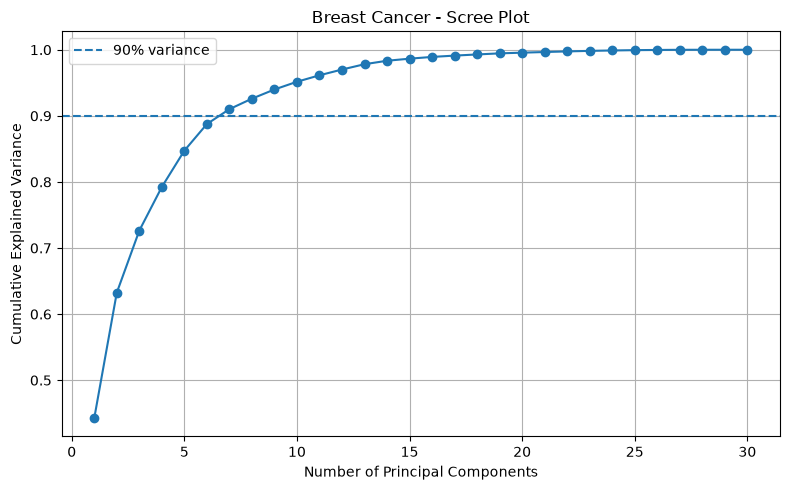
\includegraphics[width=\columnwidth]{./../figures/pca_breast.png}
\caption{PCA analysis on Breast Cancer: Scree plot showing cumulative explained variance and 2D projection with true labels, K-Means labels, and DBSCAN labels.}
\label{fig:pca_bc}
\end{figure}

\begin{figure}[h]
\centering
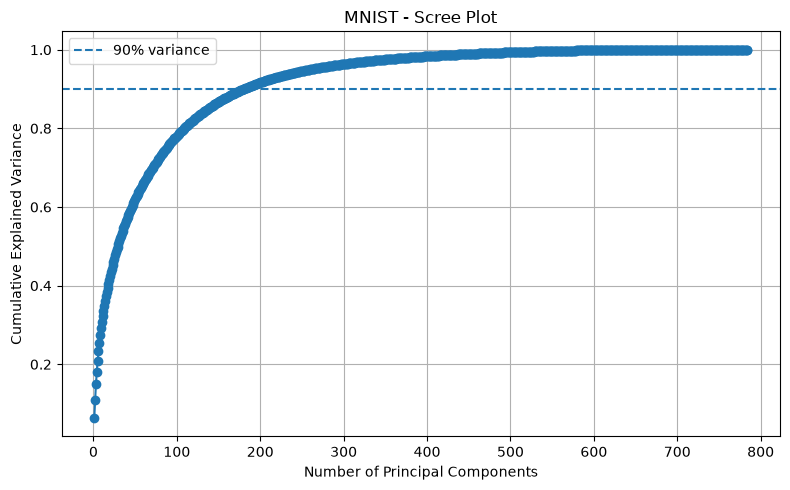
\includegraphics[width=\columnwidth]{./../figures/pca_mnist.png}
\caption{PCA analysis on MNIST: The first two components explain only 10.82\% of variance, and digit clusters show substantial overlap in PCA space.}
\label{fig:pca_mnist}
\end{figure}

\begin{figure}[h]
\centering
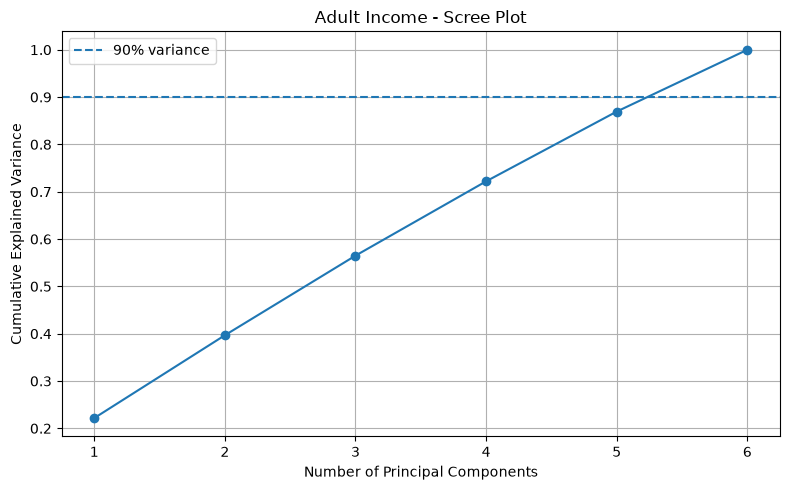
\includegraphics[width=\columnwidth]{./../figures/pca_Adult.png}
\caption{PCA analysis on Adult Income: The two classes ($\leq$50K and $>$50K) overlap substantially in PCA space, explaining the modest supervised learning performance.}
\label{fig:pca_adult}
\end{figure}

\section{Experiment 9: K-Means and DBSCAN Clustering}

Unsupervised clustering methods are evaluated using Adjusted Rand Index (ARI), which measures agreement between clustering assignments and true labels, adjusted for chance.

\subsection{K-Means Results}

K-Means is evaluated for $k = 1, \ldots, 10$ with 10 random restarts per $k$, selecting the configuration with lowest inertia.

\begin{table}[h]
\centering
\caption{K-Means optimal clustering results by ARI.}
\label{tab:kmeans}
\small
\begin{tabular}{lccc}
\toprule
Dataset & Best $k$ & Inertia & Best ARI \\
\midrule
Breast Cancer & 2 & 2186.8 & 0.654 \\
Adult Income & 4 & 577,215 & 0.089 \\
Covertype & 5 & 35,923 & 0.041 \\
MNIST & 10 & 26.4$\times 10^6$ & 0.281 \\
\bottomrule
\end{tabular}
\end{table}

Breast Cancer achieves the highest ARI (0.654) at $k=2$, matching the true binary classes, confirming clear cluster structure. MNIST achieves moderate ARI (0.281) at $k=10$, indicating that digit classes form partially separable clusters in feature space. Adult Income and Covertype exhibit low ARI values (0.089 and 0.041), suggesting that supervised class boundaries do not correspond to natural cluster structure.

\begin{figure}[h]
\centering
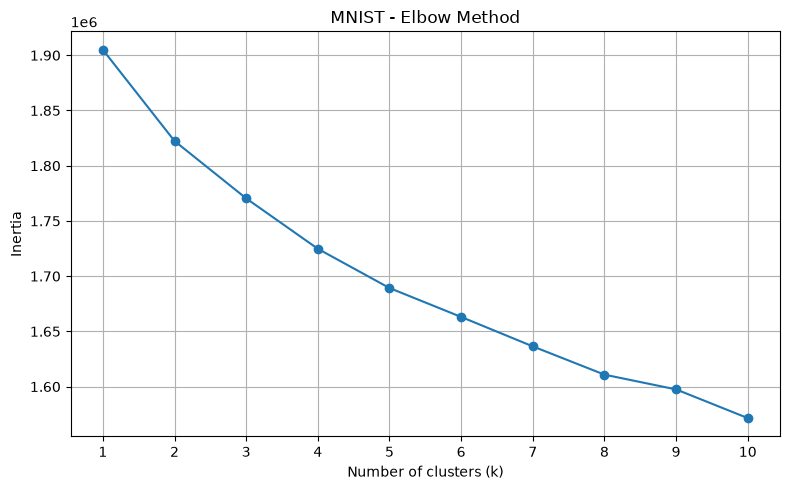
\includegraphics[width=\columnwidth]{./../figures/elbow_mnist.png}
\caption{Elbow method plot for MNIST showing inertia vs number of clusters $k$. The elbow reflecting diffuse cluster structure.}
\label{fig:elbow}
\end{figure}

\subsection{DBSCAN Results}

DBSCAN is evaluated across candidate $\epsilon$ values derived from $k$-distance plots, with results filtered to require at least 2 clusters and noise fraction $\leq$ 0.80.

\begin{table}[h]
\centering
\caption{DBSCAN optimal results from automated epsilon search.}
\label{tab:dbscan}
\small
\begin{tabular}{lccccc}
\toprule
Dataset & Best $\epsilon$ & $min\_samples$ & Clusters & ARI & Noise Fraction \\
\midrule
Breast Cancer & 2.5265 & 5 & 2 & 0.271 & 0.459 \\
Adult Income & 0.9163 & 10 & 4 & 0.153 & 0.108 \\
Covertype & 1.2788 & 10 & 6 & 0.049 & 0.251 \\
MNIST & 15.0823 & 10 & 2 & 0.059 & 0.660 \\
\bottomrule
\end{tabular}
\end{table}

\subsection{Comparison}

\begin{table}[h]
\centering
\caption{Comparison of best clustering methods by ARI.}
\label{tab:cluster_compare}
\small
\begin{tabular}{lccc}
\toprule
Dataset(Best) &KMeansARI &DBSCANARI & Better \\
\midrule
WBCDT & 0.654 & 0.271 & K-Means \\
AIDT & 0.089 & 0.153 & DBSCAN \\
Cov.Ty & 0.041 & 0.049 & DBSCAN \\
MNIST & 0.281 & 0.059 & K-Means \\
\bottomrule
\end{tabular}
\end{table}

K-Means outperforms DBSCAN on Breast Cancer and MNIST, demonstrating that datasets with approximately spherical cluster structure benefit from centroid-based partitioning. DBSCAN performs slightly better on Adult Income and Covertype, where density-based structure may align more closely with class boundaries.

However, both methods achieve modest ARI values on the larger, more complex datasets (Adult Income, Covertype, MNIST), indicating that these datasets' true class labels are not well captured by purely unsupervised clustering---at least not with these algorithms and Euclidean distance.

\begin{figure}[h]
\centering
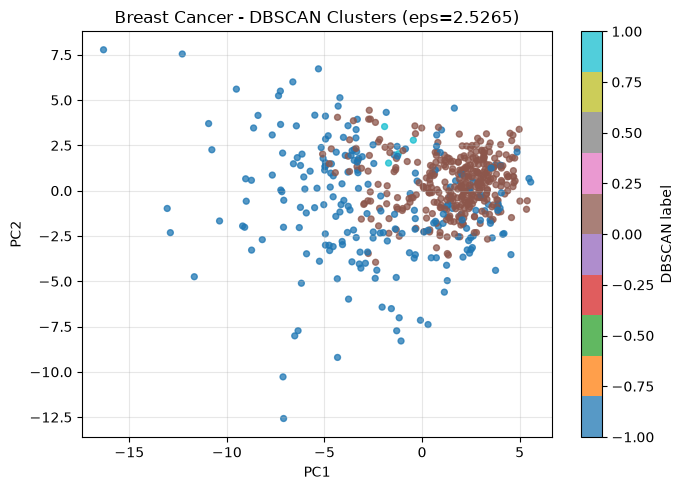
\includegraphics[width=\columnwidth]{./../figures/dbscan_breast.png}
\caption{DBSCAN clustering result on Breast Cancer ($\epsilon=2.5$, $min\_samples=5$). Two clusters are identified with 39.4\% noise fraction.}
\label{fig:dbscan_bc}
\end{figure}

\begin{figure}[h]
\centering
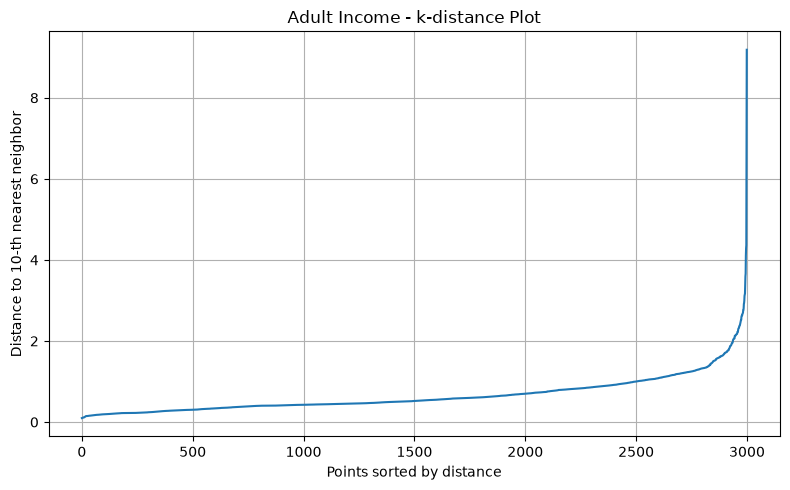
\includegraphics[width=\columnwidth]{./../figures/besteps_adult.png}
\caption{DBSCAN with optimal $\epsilon=0.9163$ on Adult Income. The K-distance plot shows the elbow region used for epsilon selection.}
\label{fig:besteps_adult}
\end{figure}

\section{Discussion}

\subsection{Implementation Validation}

Across all four datasets and multiple experimental conditions, the custom implementations consistently match scikit-learn baselines within 2\% accuracy tolerance. This validates both the algorithmic correctness and the numerical stability of the implementations. Key validation points include:
\begin{itemize}
    \item Decision Tree accuracy within 0.10\%--1.87\% of sklearn.
    \item Random Forest 5-fold CV performance closely tracking sklearn RF.
    \item Bias-variance decomposition identity verified to $<10^{-12}$ precision.
\end{itemize}

\subsection{Boosting vs Bagging: Empirical Contrasts}

The experiments consistently reveal the fundamental differences between boosting and bagging:
\begin{itemize}
    \item \textbf{Bias-Variance Trade-off}: AdaBoost achieves lower bias$^2$ (0.026 vs 0.036) while Random Forest achieves dramatically lower variance (0.002 vs 0.015), confirming the theoretical expectations.
    \item \textbf{Noise Sensitivity}: AdaBoost degrades substantially under label noise (0.098 degradation at 20\% noise on Breast Cancer) while Random Forest remains stable (0.021 degradation). AdaBoost's re-weighting mechanism amplifies the impact of mislabeled samples.
    \item \textbf{Scaling Behavior}: Both methods improve with more estimators, but AdaBoost reaches peak performance faster (20--50 estimators) while Random Forest continues improving up to 140--160 estimators.
    \item \textbf{Overfitting}: AdaBoost's training accuracy continues increasing beyond the point of test accuracy saturation, indicating eventual overfitting. Random Forest's OOB accuracy closely tracks test accuracy, providing reliable early stopping signal.
\end{itemize}

\subsection{Limitations}

The project has several acknowledged limitations:
\begin{enumerate}
    \item Computational constraints necessitated MNIST for cross-validation and scaling experiments (1,000--3,000 some experiments samples). Results may not fully reflect performance on the complete dataset.
    \item 
\end{enumerate}

\subsection{Future Work}

Potential directions for future development include:
\begin{enumerate}
    \item Implementing additional ensemble methods such as Gradient Boosting and XGBoost-style optimization.
    \item Adding spectral clustering and hierarchical clustering to the unsupervised toolkit.
    \item Implementing feature selection methods (chi-squared, mutual information).
\end{enumerate}

\section{Conclusion}

Ferocious Minsky demonstrates that implementing machine learning algorithms from scratch provides insights that are not available through library-only usage. The project's key contributions and findings are:

\begin{enumerate}
    \item Seven core machine learning algorithms---Decision Tree, Decision Stump, AdaBoost (SAMME), Random Forest, PCA, K-Means, and DBSCAN---are implemented entirely from scratch using Python and NumPy.
    \item The custom Decision Tree achieves accuracy within 2\% of scikit-learn across all four benchmark datasets, validating algorithmic correctness.
    \item Bias-variance decomposition empirically confirms that AdaBoost reduces bias ($\text{Bias}^2 = 0.026$ vs 0.036) while Random Forest reduces variance ($\text{Var} = 0.002$ vs 0.015), with the decomposition identity verified to numerical precision.
    \item Noise robustness analysis demonstrates that Random Forest degrades only 0.021 in accuracy at 20\% label noise on Breast Cancer compared to AdaBoost's 0.098 degradation, confirming that bootstrap aggregation provides inherent robustness against label corruption.
    \item Unsupervised analysis reveals that K-Means achieves the highest clustering accuracy on Breast Cancer (ARI 0.654 at $k=2$), while both K-Means and DBSCAN struggle with Adult Income and Covertype (ARI $<$ 0.15), suggesting these datasets' class boundaries do not align with natural cluster structure.
    \item PCA dimensionality reduction shows that tabular datasets require only 6--7 components for 90\% explained variance, while MNIST requires 180 components, reflecting the high intrinsic dimensionality of image data.
    \item The project includes 124 automated unit tests achieving 75\% source-code coverage, Ruff linting, MyPy type checking, and GitHub Actions continuous integration, demonstrating engineering rigor beyond algorithm implementation.
\end{enumerate}

The complete source code, experimental notebooks, figures, and documentation are organized in a modular repository structure suitable for educational use and further development. Ferocious Minsky stands as a testament to the Madagascar Penguins team's comprehensive understanding of machine learning fundamentals, from theory through implementation to empirical validation.

\section*{Acknowledgment}

The Madagascar Penguins team (Murad Tagizade, Bayram Bayramov, Ferman Khankishiyev , Mahmud Ramazanov) gratefully acknowledges the instruction and guidance provided by the AI Academy, National AI Center, during the Spring 2026 Machine Learning course. All implementations, experiments, and documentation were developed collaboratively with each team member contributing to specific modules as detailed in the Team Contribution Report.

\begin{thebibliography}{10}
\bibitem{hastie2009elements}
T. Hastie, R. Tibshirani, and J. Friedman, \emph{The Elements of Statistical Learning}, 2nd ed. New York, NY, USA: Springer, 2009.

\bibitem{breiman2001random}
L. Breiman, ``Random Forests,'' \emph{Machine Learning}, vol. 45, no. 1, pp. 5--32, 2001.

\bibitem{freund1997decision}
Y. Freund and R. E. Schapire, ``A Decision-Theoretic Generalization of On-Line Learning and an Application to Boosting,'' \emph{Journal of Computer and System Sciences}, vol. 55, no. 1, pp. 119--139, 1997.

\bibitem{zhu2009multi}
J. Zhu, H. Zou, S. Rosset, and T. Hastie, ``Multi-class AdaBoost,'' \emph{Statistics and Its Interface}, vol. 2, no. 3, pp. 349--360, 2009.

\bibitem{ester1996density}
M. Ester, H.-P. Kriegel, J. Sander, and X. Xu, ``A Density-Based Algorithm for Discovering Clusters in Large Spatial Databases with Noise,'' in \textit{Proc. 2nd Int. Conf. Knowledge Discovery and Data Mining (KDD)}, 1996, pp. 226--231.

\bibitem{lloyd1982least}
S. P. Lloyd, ``Least Squares Quantization in PCM,'' \textit{IEEE Trans. Information Theory}, vol. 28, no. 2, pp. 129--137, 1982.

\bibitem{jolliffe2002pca}
I. T. Jolliffe, \emph{Principal Component Analysis}, 2nd ed. New York, NY, USA: Springer, 2002.

\bibitem{dheeru2017uci}
D. Dheeru and E. Karra Taniskidou, ``UCI Machine Learning Repository,'' University of California, Irvine, 2017. [Online]. Available: \url{http://archive.ics.uci.edu/ml}

\bibitem{lecun1998mnist}
Y. LeCun, L. Bottou, Y. Bengio, and P. Haffner, ``Gradient-Based Learning Applied to Document Recognition,'' \textit{Proc. IEEE}, vol. 86, no. 11, pp. 2278--2324, 1998.

\bibitem{scikit-learn}
F. Pedregosa \textit{et al.}, ``Scikit-learn: Machine Learning in Python,'' \textit{Journal of Machine Learning Research}, vol. 12, pp. 2825--2830, 2011.

\end{thebibliography}

\end{document}
